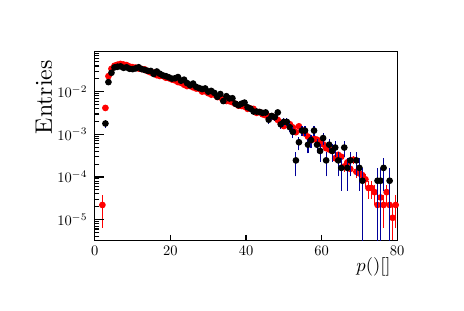
\begin{tikzpicture}
\pgfdeclareplotmark{cross} {
\pgfpathmoveto{\pgfpoint{-0.3\pgfplotmarksize}{\pgfplotmarksize}}
\pgfpathlineto{\pgfpoint{+0.3\pgfplotmarksize}{\pgfplotmarksize}}
\pgfpathlineto{\pgfpoint{+0.3\pgfplotmarksize}{0.3\pgfplotmarksize}}
\pgfpathlineto{\pgfpoint{+1\pgfplotmarksize}{0.3\pgfplotmarksize}}
\pgfpathlineto{\pgfpoint{+1\pgfplotmarksize}{-0.3\pgfplotmarksize}}
\pgfpathlineto{\pgfpoint{+0.3\pgfplotmarksize}{-0.3\pgfplotmarksize}}
\pgfpathlineto{\pgfpoint{+0.3\pgfplotmarksize}{-1.\pgfplotmarksize}}
\pgfpathlineto{\pgfpoint{-0.3\pgfplotmarksize}{-1.\pgfplotmarksize}}
\pgfpathlineto{\pgfpoint{-0.3\pgfplotmarksize}{-0.3\pgfplotmarksize}}
\pgfpathlineto{\pgfpoint{-1.\pgfplotmarksize}{-0.3\pgfplotmarksize}}
\pgfpathlineto{\pgfpoint{-1.\pgfplotmarksize}{0.3\pgfplotmarksize}}
\pgfpathlineto{\pgfpoint{-0.3\pgfplotmarksize}{0.3\pgfplotmarksize}}
\pgfpathclose
\pgfusepathqstroke
}
\pgfdeclareplotmark{cross*} {
\pgfpathmoveto{\pgfpoint{-0.3\pgfplotmarksize}{\pgfplotmarksize}}
\pgfpathlineto{\pgfpoint{+0.3\pgfplotmarksize}{\pgfplotmarksize}}
\pgfpathlineto{\pgfpoint{+0.3\pgfplotmarksize}{0.3\pgfplotmarksize}}
\pgfpathlineto{\pgfpoint{+1\pgfplotmarksize}{0.3\pgfplotmarksize}}
\pgfpathlineto{\pgfpoint{+1\pgfplotmarksize}{-0.3\pgfplotmarksize}}
\pgfpathlineto{\pgfpoint{+0.3\pgfplotmarksize}{-0.3\pgfplotmarksize}}
\pgfpathlineto{\pgfpoint{+0.3\pgfplotmarksize}{-1.\pgfplotmarksize}}
\pgfpathlineto{\pgfpoint{-0.3\pgfplotmarksize}{-1.\pgfplotmarksize}}
\pgfpathlineto{\pgfpoint{-0.3\pgfplotmarksize}{-0.3\pgfplotmarksize}}
\pgfpathlineto{\pgfpoint{-1.\pgfplotmarksize}{-0.3\pgfplotmarksize}}
\pgfpathlineto{\pgfpoint{-1.\pgfplotmarksize}{0.3\pgfplotmarksize}}
\pgfpathlineto{\pgfpoint{-0.3\pgfplotmarksize}{0.3\pgfplotmarksize}}
\pgfpathclose
\pgfusepathqfillstroke
}
\pgfdeclareplotmark{newstar} {
\pgfpathmoveto{\pgfqpoint{0pt}{\pgfplotmarksize}}
\pgfpathlineto{\pgfqpointpolar{44}{0.5\pgfplotmarksize}}
\pgfpathlineto{\pgfqpointpolar{18}{\pgfplotmarksize}}
\pgfpathlineto{\pgfqpointpolar{-20}{0.5\pgfplotmarksize}}
\pgfpathlineto{\pgfqpointpolar{-54}{\pgfplotmarksize}}
\pgfpathlineto{\pgfqpointpolar{-90}{0.5\pgfplotmarksize}}
\pgfpathlineto{\pgfqpointpolar{234}{\pgfplotmarksize}}
\pgfpathlineto{\pgfqpointpolar{198}{0.5\pgfplotmarksize}}
\pgfpathlineto{\pgfqpointpolar{162}{\pgfplotmarksize}}
\pgfpathlineto{\pgfqpointpolar{134}{0.5\pgfplotmarksize}}
\pgfpathclose
\pgfusepathqstroke
}
\pgfdeclareplotmark{newstar*} {
\pgfpathmoveto{\pgfqpoint{0pt}{\pgfplotmarksize}}
\pgfpathlineto{\pgfqpointpolar{44}{0.5\pgfplotmarksize}}
\pgfpathlineto{\pgfqpointpolar{18}{\pgfplotmarksize}}
\pgfpathlineto{\pgfqpointpolar{-20}{0.5\pgfplotmarksize}}
\pgfpathlineto{\pgfqpointpolar{-54}{\pgfplotmarksize}}
\pgfpathlineto{\pgfqpointpolar{-90}{0.5\pgfplotmarksize}}
\pgfpathlineto{\pgfqpointpolar{234}{\pgfplotmarksize}}
\pgfpathlineto{\pgfqpointpolar{198}{0.5\pgfplotmarksize}}
\pgfpathlineto{\pgfqpointpolar{162}{\pgfplotmarksize}}
\pgfpathlineto{\pgfqpointpolar{134}{0.5\pgfplotmarksize}}
\pgfpathclose
\pgfusepathqfillstroke
}
\definecolor{c}{rgb}{1,1,1};
\draw [color=c, fill=c] (0.1,3.18322) rectangle (4.9,6.17919);
\draw [color=c, fill=c] (0.58,3.48282) rectangle (4.42,5.8796);
\definecolor{c}{rgb}{0,0,0};
\draw [c] (0.58,3.48282) -- (0.58,5.8796) -- (4.42,5.8796) -- (4.42,3.48282) -- (0.58,3.48282);
\definecolor{c}{rgb}{1,0,0};
\draw [c] (0.676,3.64579) -- (0.676,3.93449);
\draw [c] (0.676,3.93449) -- (0.676,4.06023);
\draw [c] (0.6568,3.93449) -- (0.676,3.93449);
\draw [c] (0.676,3.93449) -- (0.6952,3.93449);
\foreach \P in {(0.676,3.93449)}{\draw[mark options={color=c,fill=c},mark size=2.402402pt,mark=*,mark size=1pt] plot coordinates {\P};}
\draw [c] (0.7144,5.15447) -- (0.7144,5.16688);
\draw [c] (0.7144,5.16688) -- (0.7144,5.17868);
\draw [c] (0.6952,5.16688) -- (0.7144,5.16688);
\draw [c] (0.7144,5.16688) -- (0.7336,5.16688);
\foreach \P in {(0.7144,5.16688)}{\draw[mark options={color=c,fill=c},mark size=2.402402pt,mark=*,mark size=1pt] plot coordinates {\P};}
\draw [c] (0.7528,5.56487) -- (0.7528,5.57005);
\draw [c] (0.7528,5.57005) -- (0.7528,5.57513);
\draw [c] (0.7336,5.57005) -- (0.7528,5.57005);
\draw [c] (0.7528,5.57005) -- (0.772,5.57005);
\foreach \P in {(0.7528,5.57005)}{\draw[mark options={color=c,fill=c},mark size=2.402402pt,mark=*,mark size=1pt] plot coordinates {\P};}
\draw [c] (0.7912,5.65934) -- (0.7912,5.66358);
\draw [c] (0.7912,5.66358) -- (0.7912,5.66775);
\draw [c] (0.772,5.66358) -- (0.7912,5.66358);
\draw [c] (0.7912,5.66358) -- (0.8104,5.66358);
\foreach \P in {(0.7912,5.66358)}{\draw[mark options={color=c,fill=c},mark size=2.402402pt,mark=*,mark size=1pt] plot coordinates {\P};}
\draw [c] (0.8296,5.69913) -- (0.8296,5.70303);
\draw [c] (0.8296,5.70303) -- (0.8296,5.70686);
\draw [c] (0.8104,5.70303) -- (0.8296,5.70303);
\draw [c] (0.8296,5.70303) -- (0.8488,5.70303);
\foreach \P in {(0.8296,5.70303)}{\draw[mark options={color=c,fill=c},mark size=2.402402pt,mark=*,mark size=1pt] plot coordinates {\P};}
\draw [c] (0.868,5.71265) -- (0.868,5.71644);
\draw [c] (0.868,5.71644) -- (0.868,5.72017);
\draw [c] (0.8488,5.71644) -- (0.868,5.71644);
\draw [c] (0.868,5.71644) -- (0.8872,5.71644);
\foreach \P in {(0.868,5.71644)}{\draw[mark options={color=c,fill=c},mark size=2.402402pt,mark=*,mark size=1pt] plot coordinates {\P};}
\draw [c] (0.9064,5.72197) -- (0.9064,5.72569);
\draw [c] (0.9064,5.72569) -- (0.9064,5.72934);
\draw [c] (0.8872,5.72569) -- (0.9064,5.72569);
\draw [c] (0.9064,5.72569) -- (0.9256,5.72569);
\foreach \P in {(0.9064,5.72569)}{\draw[mark options={color=c,fill=c},mark size=2.402402pt,mark=*,mark size=1pt] plot coordinates {\P};}
\draw [c] (0.9448,5.71458) -- (0.9448,5.71835);
\draw [c] (0.9448,5.71835) -- (0.9448,5.72207);
\draw [c] (0.9256,5.71835) -- (0.9448,5.71835);
\draw [c] (0.9448,5.71835) -- (0.964,5.71835);
\foreach \P in {(0.9448,5.71835)}{\draw[mark options={color=c,fill=c},mark size=2.402402pt,mark=*,mark size=1pt] plot coordinates {\P};}
\draw [c] (0.9832,5.70695) -- (0.9832,5.71079);
\draw [c] (0.9832,5.71079) -- (0.9832,5.71456);
\draw [c] (0.964,5.71079) -- (0.9832,5.71079);
\draw [c] (0.9832,5.71079) -- (1.0024,5.71079);
\foreach \P in {(0.9832,5.71079)}{\draw[mark options={color=c,fill=c},mark size=2.402402pt,mark=*,mark size=1pt] plot coordinates {\P};}
\draw [c] (1.0216,5.68877) -- (1.0216,5.69276);
\draw [c] (1.0216,5.69276) -- (1.0216,5.69668);
\draw [c] (1.0024,5.69276) -- (1.0216,5.69276);
\draw [c] (1.0216,5.69276) -- (1.0408,5.69276);
\foreach \P in {(1.0216,5.69276)}{\draw[mark options={color=c,fill=c},mark size=2.402402pt,mark=*,mark size=1pt] plot coordinates {\P};}
\draw [c] (1.06,5.68011) -- (1.06,5.68417);
\draw [c] (1.06,5.68417) -- (1.06,5.68816);
\draw [c] (1.0408,5.68417) -- (1.06,5.68417);
\draw [c] (1.06,5.68417) -- (1.0792,5.68417);
\foreach \P in {(1.06,5.68417)}{\draw[mark options={color=c,fill=c},mark size=2.402402pt,mark=*,mark size=1pt] plot coordinates {\P};}
\draw [c] (1.0984,5.67512) -- (1.0984,5.67922);
\draw [c] (1.0984,5.67922) -- (1.0984,5.68326);
\draw [c] (1.0792,5.67922) -- (1.0984,5.67922);
\draw [c] (1.0984,5.67922) -- (1.1176,5.67922);
\foreach \P in {(1.0984,5.67922)}{\draw[mark options={color=c,fill=c},mark size=2.402402pt,mark=*,mark size=1pt] plot coordinates {\P};}
\draw [c] (1.1368,5.66281) -- (1.1368,5.66702);
\draw [c] (1.1368,5.66702) -- (1.1368,5.67116);
\draw [c] (1.1176,5.66702) -- (1.1368,5.66702);
\draw [c] (1.1368,5.66702) -- (1.156,5.66702);
\foreach \P in {(1.1368,5.66702)}{\draw[mark options={color=c,fill=c},mark size=2.402402pt,mark=*,mark size=1pt] plot coordinates {\P};}
\draw [c] (1.1752,5.65682) -- (1.1752,5.66109);
\draw [c] (1.1752,5.66109) -- (1.1752,5.66528);
\draw [c] (1.156,5.66109) -- (1.1752,5.66109);
\draw [c] (1.1752,5.66109) -- (1.1944,5.66109);
\foreach \P in {(1.1752,5.66109)}{\draw[mark options={color=c,fill=c},mark size=2.402402pt,mark=*,mark size=1pt] plot coordinates {\P};}
\draw [c] (1.2136,5.65139) -- (1.2136,5.65571);
\draw [c] (1.2136,5.65571) -- (1.2136,5.65995);
\draw [c] (1.1944,5.65571) -- (1.2136,5.65571);
\draw [c] (1.2136,5.65571) -- (1.2328,5.65571);
\foreach \P in {(1.2136,5.65571)}{\draw[mark options={color=c,fill=c},mark size=2.402402pt,mark=*,mark size=1pt] plot coordinates {\P};}
\draw [c] (1.252,5.6291) -- (1.252,5.63363);
\draw [c] (1.252,5.63363) -- (1.252,5.63806);
\draw [c] (1.2328,5.63363) -- (1.252,5.63363);
\draw [c] (1.252,5.63363) -- (1.2712,5.63363);
\foreach \P in {(1.252,5.63363)}{\draw[mark options={color=c,fill=c},mark size=2.402402pt,mark=*,mark size=1pt] plot coordinates {\P};}
\draw [c] (1.2904,5.61248) -- (1.2904,5.61717);
\draw [c] (1.2904,5.61717) -- (1.2904,5.62177);
\draw [c] (1.2712,5.61717) -- (1.2904,5.61717);
\draw [c] (1.2904,5.61717) -- (1.3096,5.61717);
\foreach \P in {(1.2904,5.61717)}{\draw[mark options={color=c,fill=c},mark size=2.402402pt,mark=*,mark size=1pt] plot coordinates {\P};}
\draw [c] (1.3288,5.6095) -- (1.3288,5.61422);
\draw [c] (1.3288,5.61422) -- (1.3288,5.61885);
\draw [c] (1.3096,5.61422) -- (1.3288,5.61422);
\draw [c] (1.3288,5.61422) -- (1.348,5.61422);
\foreach \P in {(1.3288,5.61422)}{\draw[mark options={color=c,fill=c},mark size=2.402402pt,mark=*,mark size=1pt] plot coordinates {\P};}
\draw [c] (1.3672,5.57754) -- (1.3672,5.58259);
\draw [c] (1.3672,5.58259) -- (1.3672,5.58753);
\draw [c] (1.348,5.58259) -- (1.3672,5.58259);
\draw [c] (1.3672,5.58259) -- (1.3864,5.58259);
\foreach \P in {(1.3672,5.58259)}{\draw[mark options={color=c,fill=c},mark size=2.402402pt,mark=*,mark size=1pt] plot coordinates {\P};}
\draw [c] (1.4056,5.56723) -- (1.4056,5.57239);
\draw [c] (1.4056,5.57239) -- (1.4056,5.57744);
\draw [c] (1.3864,5.57239) -- (1.4056,5.57239);
\draw [c] (1.4056,5.57239) -- (1.4248,5.57239);
\foreach \P in {(1.4056,5.57239)}{\draw[mark options={color=c,fill=c},mark size=2.402402pt,mark=*,mark size=1pt] plot coordinates {\P};}
\draw [c] (1.444,5.56633) -- (1.444,5.5715);
\draw [c] (1.444,5.5715) -- (1.444,5.57656);
\draw [c] (1.4248,5.5715) -- (1.444,5.5715);
\draw [c] (1.444,5.5715) -- (1.4632,5.5715);
\foreach \P in {(1.444,5.5715)}{\draw[mark options={color=c,fill=c},mark size=2.402402pt,mark=*,mark size=1pt] plot coordinates {\P};}
\draw [c] (1.4824,5.54467) -- (1.4824,5.55008);
\draw [c] (1.4824,5.55008) -- (1.4824,5.55538);
\draw [c] (1.4632,5.55008) -- (1.4824,5.55008);
\draw [c] (1.4824,5.55008) -- (1.5016,5.55008);
\foreach \P in {(1.4824,5.55008)}{\draw[mark options={color=c,fill=c},mark size=2.402402pt,mark=*,mark size=1pt] plot coordinates {\P};}
\draw [c] (1.5208,5.5388) -- (1.5208,5.54428);
\draw [c] (1.5208,5.54428) -- (1.5208,5.54964);
\draw [c] (1.5016,5.54428) -- (1.5208,5.54428);
\draw [c] (1.5208,5.54428) -- (1.54,5.54428);
\foreach \P in {(1.5208,5.54428)}{\draw[mark options={color=c,fill=c},mark size=2.402402pt,mark=*,mark size=1pt] plot coordinates {\P};}
\draw [c] (1.5592,5.52218) -- (1.5592,5.52786);
\draw [c] (1.5592,5.52786) -- (1.5592,5.5334);
\draw [c] (1.54,5.52786) -- (1.5592,5.52786);
\draw [c] (1.5592,5.52786) -- (1.5784,5.52786);
\foreach \P in {(1.5592,5.52786)}{\draw[mark options={color=c,fill=c},mark size=2.402402pt,mark=*,mark size=1pt] plot coordinates {\P};}
\draw [c] (1.5976,5.51136) -- (1.5976,5.51717);
\draw [c] (1.5976,5.51717) -- (1.5976,5.52284);
\draw [c] (1.5784,5.51717) -- (1.5976,5.51717);
\draw [c] (1.5976,5.51717) -- (1.6168,5.51717);
\foreach \P in {(1.5976,5.51717)}{\draw[mark options={color=c,fill=c},mark size=2.402402pt,mark=*,mark size=1pt] plot coordinates {\P};}
\draw [c] (1.636,5.4892) -- (1.636,5.49529);
\draw [c] (1.636,5.49529) -- (1.636,5.50123);
\draw [c] (1.6168,5.49529) -- (1.636,5.49529);
\draw [c] (1.636,5.49529) -- (1.6552,5.49529);
\foreach \P in {(1.636,5.49529)}{\draw[mark options={color=c,fill=c},mark size=2.402402pt,mark=*,mark size=1pt] plot coordinates {\P};}
\draw [c] (1.6744,5.47949) -- (1.6744,5.48571);
\draw [c] (1.6744,5.48571) -- (1.6744,5.49177);
\draw [c] (1.6552,5.48571) -- (1.6744,5.48571);
\draw [c] (1.6744,5.48571) -- (1.6936,5.48571);
\foreach \P in {(1.6744,5.48571)}{\draw[mark options={color=c,fill=c},mark size=2.402402pt,mark=*,mark size=1pt] plot coordinates {\P};}
\draw [c] (1.7128,5.45559) -- (1.7128,5.46213);
\draw [c] (1.7128,5.46213) -- (1.7128,5.4685);
\draw [c] (1.6936,5.46213) -- (1.7128,5.46213);
\draw [c] (1.7128,5.46213) -- (1.732,5.46213);
\foreach \P in {(1.7128,5.46213)}{\draw[mark options={color=c,fill=c},mark size=2.402402pt,mark=*,mark size=1pt] plot coordinates {\P};}
\draw [c] (1.7512,5.4371) -- (1.7512,5.4439);
\draw [c] (1.7512,5.4439) -- (1.7512,5.45052);
\draw [c] (1.732,5.4439) -- (1.7512,5.4439);
\draw [c] (1.7512,5.4439) -- (1.7704,5.4439);
\foreach \P in {(1.7512,5.4439)}{\draw[mark options={color=c,fill=c},mark size=2.402402pt,mark=*,mark size=1pt] plot coordinates {\P};}
\draw [c] (1.7896,5.43845) -- (1.7896,5.44524);
\draw [c] (1.7896,5.44524) -- (1.7896,5.45184);
\draw [c] (1.7704,5.44524) -- (1.7896,5.44524);
\draw [c] (1.7896,5.44524) -- (1.8088,5.44524);
\foreach \P in {(1.7896,5.44524)}{\draw[mark options={color=c,fill=c},mark size=2.402402pt,mark=*,mark size=1pt] plot coordinates {\P};}
\draw [c] (1.828,5.42081) -- (1.828,5.42786);
\draw [c] (1.828,5.42786) -- (1.828,5.4347);
\draw [c] (1.8088,5.42786) -- (1.828,5.42786);
\draw [c] (1.828,5.42786) -- (1.8472,5.42786);
\foreach \P in {(1.828,5.42786)}{\draw[mark options={color=c,fill=c},mark size=2.402402pt,mark=*,mark size=1pt] plot coordinates {\P};}
\draw [c] (1.8664,5.406) -- (1.8664,5.41327);
\draw [c] (1.8664,5.41327) -- (1.8664,5.42033);
\draw [c] (1.8472,5.41327) -- (1.8664,5.41327);
\draw [c] (1.8664,5.41327) -- (1.8856,5.41327);
\foreach \P in {(1.8664,5.41327)}{\draw[mark options={color=c,fill=c},mark size=2.402402pt,mark=*,mark size=1pt] plot coordinates {\P};}
\draw [c] (1.9048,5.40221) -- (1.9048,5.40954);
\draw [c] (1.9048,5.40954) -- (1.9048,5.41665);
\draw [c] (1.8856,5.40954) -- (1.9048,5.40954);
\draw [c] (1.9048,5.40954) -- (1.924,5.40954);
\foreach \P in {(1.9048,5.40954)}{\draw[mark options={color=c,fill=c},mark size=2.402402pt,mark=*,mark size=1pt] plot coordinates {\P};}
\draw [c] (1.9432,5.36656) -- (1.9432,5.37447);
\draw [c] (1.9432,5.37447) -- (1.9432,5.38212);
\draw [c] (1.924,5.37447) -- (1.9432,5.37447);
\draw [c] (1.9432,5.37447) -- (1.9624,5.37447);
\foreach \P in {(1.9432,5.37447)}{\draw[mark options={color=c,fill=c},mark size=2.402402pt,mark=*,mark size=1pt] plot coordinates {\P};}
\draw [c] (1.9816,5.36943) -- (1.9816,5.37729);
\draw [c] (1.9816,5.37729) -- (1.9816,5.38489);
\draw [c] (1.9624,5.37729) -- (1.9816,5.37729);
\draw [c] (1.9816,5.37729) -- (2.0008,5.37729);
\foreach \P in {(1.9816,5.37729)}{\draw[mark options={color=c,fill=c},mark size=2.402402pt,mark=*,mark size=1pt] plot coordinates {\P};}
\draw [c] (2.02,5.34551) -- (2.02,5.35378);
\draw [c] (2.02,5.35378) -- (2.02,5.36177);
\draw [c] (2.0008,5.35378) -- (2.02,5.35378);
\draw [c] (2.02,5.35378) -- (2.0392,5.35378);
\foreach \P in {(2.02,5.35378)}{\draw[mark options={color=c,fill=c},mark size=2.402402pt,mark=*,mark size=1pt] plot coordinates {\P};}
\draw [c] (2.0584,5.32709) -- (2.0584,5.33569);
\draw [c] (2.0584,5.33569) -- (2.0584,5.34398);
\draw [c] (2.0392,5.33569) -- (2.0584,5.33569);
\draw [c] (2.0584,5.33569) -- (2.0776,5.33569);
\foreach \P in {(2.0584,5.33569)}{\draw[mark options={color=c,fill=c},mark size=2.402402pt,mark=*,mark size=1pt] plot coordinates {\P};}
\draw [c] (2.0968,5.3277) -- (2.0968,5.33629);
\draw [c] (2.0968,5.33629) -- (2.0968,5.34458);
\draw [c] (2.0776,5.33629) -- (2.0968,5.33629);
\draw [c] (2.0968,5.33629) -- (2.116,5.33629);
\foreach \P in {(2.0968,5.33629)}{\draw[mark options={color=c,fill=c},mark size=2.402402pt,mark=*,mark size=1pt] plot coordinates {\P};}
\draw [c] (2.1352,5.2968) -- (2.1352,5.30598);
\draw [c] (2.1352,5.30598) -- (2.1352,5.31481);
\draw [c] (2.116,5.30598) -- (2.1352,5.30598);
\draw [c] (2.1352,5.30598) -- (2.1544,5.30598);
\foreach \P in {(2.1352,5.30598)}{\draw[mark options={color=c,fill=c},mark size=2.402402pt,mark=*,mark size=1pt] plot coordinates {\P};}
\draw [c] (2.1736,5.29112) -- (2.1736,5.3004);
\draw [c] (2.1736,5.3004) -- (2.1736,5.30934);
\draw [c] (2.1544,5.3004) -- (2.1736,5.3004);
\draw [c] (2.1736,5.3004) -- (2.1928,5.3004);
\foreach \P in {(2.1736,5.3004)}{\draw[mark options={color=c,fill=c},mark size=2.402402pt,mark=*,mark size=1pt] plot coordinates {\P};}
\draw [c] (2.212,5.25297) -- (2.212,5.26304);
\draw [c] (2.212,5.26304) -- (2.212,5.2727);
\draw [c] (2.1928,5.26304) -- (2.212,5.26304);
\draw [c] (2.212,5.26304) -- (2.2312,5.26304);
\foreach \P in {(2.212,5.26304)}{\draw[mark options={color=c,fill=c},mark size=2.402402pt,mark=*,mark size=1pt] plot coordinates {\P};}
\draw [c] (2.2504,5.24525) -- (2.2504,5.25548);
\draw [c] (2.2504,5.25548) -- (2.2504,5.26529);
\draw [c] (2.2312,5.25548) -- (2.2504,5.25548);
\draw [c] (2.2504,5.25548) -- (2.2696,5.25548);
\foreach \P in {(2.2504,5.25548)}{\draw[mark options={color=c,fill=c},mark size=2.402402pt,mark=*,mark size=1pt] plot coordinates {\P};}
\draw [c] (2.2888,5.24173) -- (2.2888,5.25205);
\draw [c] (2.2888,5.25205) -- (2.2888,5.26192);
\draw [c] (2.2696,5.25205) -- (2.2888,5.25205);
\draw [c] (2.2888,5.25205) -- (2.308,5.25205);
\foreach \P in {(2.2888,5.25205)}{\draw[mark options={color=c,fill=c},mark size=2.402402pt,mark=*,mark size=1pt] plot coordinates {\P};}
\draw [c] (2.3272,5.229) -- (2.3272,5.2396);
\draw [c] (2.3272,5.2396) -- (2.3272,5.24974);
\draw [c] (2.308,5.2396) -- (2.3272,5.2396);
\draw [c] (2.3272,5.2396) -- (2.3464,5.2396);
\foreach \P in {(2.3272,5.2396)}{\draw[mark options={color=c,fill=c},mark size=2.402402pt,mark=*,mark size=1pt] plot coordinates {\P};}
\draw [c] (2.3656,5.20802) -- (2.3656,5.2191);
\draw [c] (2.3656,5.2191) -- (2.3656,5.22968);
\draw [c] (2.3464,5.2191) -- (2.3656,5.2191);
\draw [c] (2.3656,5.2191) -- (2.3848,5.2191);
\foreach \P in {(2.3656,5.2191)}{\draw[mark options={color=c,fill=c},mark size=2.402402pt,mark=*,mark size=1pt] plot coordinates {\P};}
\draw [c] (2.404,5.18388) -- (2.404,5.19554);
\draw [c] (2.404,5.19554) -- (2.404,5.20665);
\draw [c] (2.3848,5.19554) -- (2.404,5.19554);
\draw [c] (2.404,5.19554) -- (2.4232,5.19554);
\foreach \P in {(2.404,5.19554)}{\draw[mark options={color=c,fill=c},mark size=2.402402pt,mark=*,mark size=1pt] plot coordinates {\P};}
\draw [c] (2.4424,5.18104) -- (2.4424,5.19277);
\draw [c] (2.4424,5.19277) -- (2.4424,5.20395);
\draw [c] (2.4232,5.19277) -- (2.4424,5.19277);
\draw [c] (2.4424,5.19277) -- (2.4616,5.19277);
\foreach \P in {(2.4424,5.19277)}{\draw[mark options={color=c,fill=c},mark size=2.402402pt,mark=*,mark size=1pt] plot coordinates {\P};}
\draw [c] (2.4808,5.17172) -- (2.4808,5.18369);
\draw [c] (2.4808,5.18369) -- (2.4808,5.19507);
\draw [c] (2.4616,5.18369) -- (2.4808,5.18369);
\draw [c] (2.4808,5.18369) -- (2.5,5.18369);
\foreach \P in {(2.4808,5.18369)}{\draw[mark options={color=c,fill=c},mark size=2.402402pt,mark=*,mark size=1pt] plot coordinates {\P};}
\draw [c] (2.5192,5.14335) -- (2.5192,5.15607);
\draw [c] (2.5192,5.15607) -- (2.5192,5.16813);
\draw [c] (2.5,5.15607) -- (2.5192,5.15607);
\draw [c] (2.5192,5.15607) -- (2.5384,5.15607);
\foreach \P in {(2.5192,5.15607)}{\draw[mark options={color=c,fill=c},mark size=2.402402pt,mark=*,mark size=1pt] plot coordinates {\P};}
\draw [c] (2.5576,5.14734) -- (2.5576,5.15994);
\draw [c] (2.5576,5.15994) -- (2.5576,5.1719);
\draw [c] (2.5384,5.15994) -- (2.5576,5.15994);
\draw [c] (2.5576,5.15994) -- (2.5768,5.15994);
\foreach \P in {(2.5576,5.15994)}{\draw[mark options={color=c,fill=c},mark size=2.402402pt,mark=*,mark size=1pt] plot coordinates {\P};}
\draw [c] (2.596,5.14134) -- (2.596,5.1541);
\draw [c] (2.596,5.1541) -- (2.596,5.16621);
\draw [c] (2.5768,5.1541) -- (2.596,5.1541);
\draw [c] (2.596,5.1541) -- (2.6152,5.1541);
\foreach \P in {(2.596,5.1541)}{\draw[mark options={color=c,fill=c},mark size=2.402402pt,mark=*,mark size=1pt] plot coordinates {\P};}
\draw [c] (2.6344,5.09035) -- (2.6344,5.10458);
\draw [c] (2.6344,5.10458) -- (2.6344,5.11799);
\draw [c] (2.6152,5.10458) -- (2.6344,5.10458);
\draw [c] (2.6344,5.10458) -- (2.6536,5.10458);
\foreach \P in {(2.6344,5.10458)}{\draw[mark options={color=c,fill=c},mark size=2.402402pt,mark=*,mark size=1pt] plot coordinates {\P};}
\draw [c] (2.6728,5.09937) -- (2.6728,5.11333);
\draw [c] (2.6728,5.11333) -- (2.6728,5.12651);
\draw [c] (2.6536,5.11333) -- (2.6728,5.11333);
\draw [c] (2.6728,5.11333) -- (2.692,5.11333);
\foreach \P in {(2.6728,5.11333)}{\draw[mark options={color=c,fill=c},mark size=2.402402pt,mark=*,mark size=1pt] plot coordinates {\P};}
\draw [c] (2.7112,5.07121) -- (2.7112,5.08603);
\draw [c] (2.7112,5.08603) -- (2.7112,5.09997);
\draw [c] (2.692,5.08603) -- (2.7112,5.08603);
\draw [c] (2.7112,5.08603) -- (2.7304,5.08603);
\foreach \P in {(2.7112,5.08603)}{\draw[mark options={color=c,fill=c},mark size=2.402402pt,mark=*,mark size=1pt] plot coordinates {\P};}
\draw [c] (2.7496,5.05722) -- (2.7496,5.07249);
\draw [c] (2.7496,5.07249) -- (2.7496,5.08682);
\draw [c] (2.7304,5.07249) -- (2.7496,5.07249);
\draw [c] (2.7496,5.07249) -- (2.7688,5.07249);
\foreach \P in {(2.7496,5.07249)}{\draw[mark options={color=c,fill=c},mark size=2.402402pt,mark=*,mark size=1pt] plot coordinates {\P};}
\draw [c] (2.788,5.04541) -- (2.788,5.06106);
\draw [c] (2.788,5.06106) -- (2.788,5.07574);
\draw [c] (2.7688,5.06106) -- (2.788,5.06106);
\draw [c] (2.788,5.06106) -- (2.8072,5.06106);
\foreach \P in {(2.788,5.06106)}{\draw[mark options={color=c,fill=c},mark size=2.402402pt,mark=*,mark size=1pt] plot coordinates {\P};}
\draw [c] (2.8264,5.04641) -- (2.8264,5.06204);
\draw [c] (2.8264,5.06204) -- (2.8264,5.07668);
\draw [c] (2.8072,5.06204) -- (2.8264,5.06204);
\draw [c] (2.8264,5.06204) -- (2.8456,5.06204);
\foreach \P in {(2.8264,5.06204)}{\draw[mark options={color=c,fill=c},mark size=2.402402pt,mark=*,mark size=1pt] plot coordinates {\P};}
\draw [c] (2.8648,5.03191) -- (2.8648,5.04802);
\draw [c] (2.8648,5.04802) -- (2.8648,5.0631);
\draw [c] (2.8456,5.04802) -- (2.8648,5.04802);
\draw [c] (2.8648,5.04802) -- (2.884,5.04802);
\foreach \P in {(2.8648,5.04802)}{\draw[mark options={color=c,fill=c},mark size=2.402402pt,mark=*,mark size=1pt] plot coordinates {\P};}
\draw [c] (2.9032,4.99752) -- (2.9032,5.01486);
\draw [c] (2.9032,5.01486) -- (2.9032,5.031);
\draw [c] (2.884,5.01486) -- (2.9032,5.01486);
\draw [c] (2.9032,5.01486) -- (2.9224,5.01486);
\foreach \P in {(2.9032,5.01486)}{\draw[mark options={color=c,fill=c},mark size=2.402402pt,mark=*,mark size=1pt] plot coordinates {\P};}
\draw [c] (2.9416,4.94995) -- (2.9416,4.96912);
\draw [c] (2.9416,4.96912) -- (2.9416,4.98685);
\draw [c] (2.9224,4.96912) -- (2.9416,4.96912);
\draw [c] (2.9416,4.96912) -- (2.9608,4.96912);
\foreach \P in {(2.9416,4.96912)}{\draw[mark options={color=c,fill=c},mark size=2.402402pt,mark=*,mark size=1pt] plot coordinates {\P};}
\draw [c] (2.98,4.91609) -- (2.98,4.93669);
\draw [c] (2.98,4.93669) -- (2.98,4.95564);
\draw [c] (2.9608,4.93669) -- (2.98,4.93669);
\draw [c] (2.98,4.93669) -- (2.9992,4.93669);
\foreach \P in {(2.98,4.93669)}{\draw[mark options={color=c,fill=c},mark size=2.402402pt,mark=*,mark size=1pt] plot coordinates {\P};}
\draw [c] (3.0184,4.94075) -- (3.0184,4.9603);
\draw [c] (3.0184,4.9603) -- (3.0184,4.97836);
\draw [c] (2.9992,4.9603) -- (3.0184,4.9603);
\draw [c] (3.0184,4.9603) -- (3.0376,4.9603);
\foreach \P in {(3.0184,4.9603)}{\draw[mark options={color=c,fill=c},mark size=2.402402pt,mark=*,mark size=1pt] plot coordinates {\P};}
\draw [c] (3.0568,4.94075) -- (3.0568,4.9603);
\draw [c] (3.0568,4.9603) -- (3.0568,4.97836);
\draw [c] (3.0376,4.9603) -- (3.0568,4.9603);
\draw [c] (3.0568,4.9603) -- (3.076,4.9603);
\foreach \P in {(3.0568,4.9603)}{\draw[mark options={color=c,fill=c},mark size=2.402402pt,mark=*,mark size=1pt] plot coordinates {\P};}
\draw [c] (3.0952,4.89812) -- (3.0952,4.91953);
\draw [c] (3.0952,4.91953) -- (3.0952,4.93915);
\draw [c] (3.076,4.91953) -- (3.0952,4.91953);
\draw [c] (3.0952,4.91953) -- (3.1144,4.91953);
\foreach \P in {(3.0952,4.91953)}{\draw[mark options={color=c,fill=c},mark size=2.402402pt,mark=*,mark size=1pt] plot coordinates {\P};}
\draw [c] (3.1336,4.83439) -- (3.1336,4.85891);
\draw [c] (3.1336,4.85891) -- (3.1336,4.8811);
\draw [c] (3.1144,4.85891) -- (3.1336,4.85891);
\draw [c] (3.1336,4.85891) -- (3.1528,4.85891);
\foreach \P in {(3.1336,4.85891)}{\draw[mark options={color=c,fill=c},mark size=2.402402pt,mark=*,mark size=1pt] plot coordinates {\P};}
\draw [c] (3.172,4.9126) -- (3.172,4.93336);
\draw [c] (3.172,4.93336) -- (3.172,4.95244);
\draw [c] (3.1528,4.93336) -- (3.172,4.93336);
\draw [c] (3.172,4.93336) -- (3.1912,4.93336);
\foreach \P in {(3.172,4.93336)}{\draw[mark options={color=c,fill=c},mark size=2.402402pt,mark=*,mark size=1pt] plot coordinates {\P};}
\draw [c] (3.2104,4.86194) -- (3.2104,4.88506);
\draw [c] (3.2104,4.88506) -- (3.2104,4.90611);
\draw [c] (3.1912,4.88506) -- (3.2104,4.88506);
\draw [c] (3.2104,4.88506) -- (3.2296,4.88506);
\foreach \P in {(3.2104,4.88506)}{\draw[mark options={color=c,fill=c},mark size=2.402402pt,mark=*,mark size=1pt] plot coordinates {\P};}
\draw [c] (3.2488,4.81674) -- (3.2488,4.84219);
\draw [c] (3.2488,4.84219) -- (3.2488,4.86515);
\draw [c] (3.2296,4.84219) -- (3.2488,4.84219);
\draw [c] (3.2488,4.84219) -- (3.268,4.84219);
\foreach \P in {(3.2488,4.84219)}{\draw[mark options={color=c,fill=c},mark size=2.402402pt,mark=*,mark size=1pt] plot coordinates {\P};}
\draw [c] (3.2872,4.77391) -- (3.2872,4.80179);
\draw [c] (3.2872,4.80179) -- (3.2872,4.82671);
\draw [c] (3.268,4.80179) -- (3.2872,4.80179);
\draw [c] (3.2872,4.80179) -- (3.3064,4.80179);
\foreach \P in {(3.2872,4.80179)}{\draw[mark options={color=c,fill=c},mark size=2.402402pt,mark=*,mark size=1pt] plot coordinates {\P};}
\draw [c] (3.3256,4.72183) -- (3.3256,4.75297);
\draw [c] (3.3256,4.75297) -- (3.3256,4.78046);
\draw [c] (3.3064,4.75297) -- (3.3256,4.75297);
\draw [c] (3.3256,4.75297) -- (3.3448,4.75297);
\foreach \P in {(3.3256,4.75297)}{\draw[mark options={color=c,fill=c},mark size=2.402402pt,mark=*,mark size=1pt] plot coordinates {\P};}
\draw [c] (3.364,4.74753) -- (3.364,4.77702);
\draw [c] (3.364,4.77702) -- (3.364,4.80321);
\draw [c] (3.3448,4.77702) -- (3.364,4.77702);
\draw [c] (3.364,4.77702) -- (3.3832,4.77702);
\foreach \P in {(3.364,4.77702)}{\draw[mark options={color=c,fill=c},mark size=2.402402pt,mark=*,mark size=1pt] plot coordinates {\P};}
\draw [c] (3.4024,4.73318) -- (3.4024,4.76358);
\draw [c] (3.4024,4.76358) -- (3.4024,4.79049);
\draw [c] (3.3832,4.76358) -- (3.4024,4.76358);
\draw [c] (3.4024,4.76358) -- (3.4216,4.76358);
\foreach \P in {(3.4024,4.76358)}{\draw[mark options={color=c,fill=c},mark size=2.402402pt,mark=*,mark size=1pt] plot coordinates {\P};}
\draw [c] (3.4408,4.70993) -- (3.4408,4.74186);
\draw [c] (3.4408,4.74186) -- (3.4408,4.76997);
\draw [c] (3.4216,4.74186) -- (3.4408,4.74186);
\draw [c] (3.4408,4.74186) -- (3.46,4.74186);
\foreach \P in {(3.4408,4.74186)}{\draw[mark options={color=c,fill=c},mark size=2.402402pt,mark=*,mark size=1pt] plot coordinates {\P};}
\draw [c] (3.4792,4.67024) -- (3.4792,4.70498);
\draw [c] (3.4792,4.70498) -- (3.4792,4.73525);
\draw [c] (3.46,4.70498) -- (3.4792,4.70498);
\draw [c] (3.4792,4.70498) -- (3.4984,4.70498);
\foreach \P in {(3.4792,4.70498)}{\draw[mark options={color=c,fill=c},mark size=2.402402pt,mark=*,mark size=1pt] plot coordinates {\P};}
\draw [c] (3.5176,4.61692) -- (3.5176,4.65582);
\draw [c] (3.5176,4.65582) -- (3.5176,4.68919);
\draw [c] (3.4984,4.65582) -- (3.5176,4.65582);
\draw [c] (3.5176,4.65582) -- (3.5368,4.65582);
\foreach \P in {(3.5176,4.65582)}{\draw[mark options={color=c,fill=c},mark size=2.402402pt,mark=*,mark size=1pt] plot coordinates {\P};}
\draw [c] (3.556,4.59836) -- (3.556,4.63882);
\draw [c] (3.556,4.63882) -- (3.556,4.67333);
\draw [c] (3.5368,4.63882) -- (3.556,4.63882);
\draw [c] (3.556,4.63882) -- (3.5752,4.63882);
\foreach \P in {(3.556,4.63882)}{\draw[mark options={color=c,fill=c},mark size=2.402402pt,mark=*,mark size=1pt] plot coordinates {\P};}
\draw [c] (3.5944,4.57826) -- (3.5944,4.62049);
\draw [c] (3.5944,4.62049) -- (3.5944,4.65628);
\draw [c] (3.5752,4.62049) -- (3.5944,4.62049);
\draw [c] (3.5944,4.62049) -- (3.6136,4.62049);
\foreach \P in {(3.5944,4.62049)}{\draw[mark options={color=c,fill=c},mark size=2.402402pt,mark=*,mark size=1pt] plot coordinates {\P};}
\draw [c] (3.6328,4.47585) -- (3.6328,4.52832);
\draw [c] (3.6328,4.52832) -- (3.6328,4.57118);
\draw [c] (3.6136,4.52832) -- (3.6328,4.52832);
\draw [c] (3.6328,4.52832) -- (3.652,4.52832);
\foreach \P in {(3.6328,4.52832)}{\draw[mark options={color=c,fill=c},mark size=2.402402pt,mark=*,mark size=1pt] plot coordinates {\P};}
\draw [c] (3.6712,4.52379) -- (3.6712,4.57118);
\draw [c] (3.6712,4.57118) -- (3.6712,4.61061);
\draw [c] (3.652,4.57118) -- (3.6712,4.57118);
\draw [c] (3.6712,4.57118) -- (3.6904,4.57118);
\foreach \P in {(3.6712,4.57118)}{\draw[mark options={color=c,fill=c},mark size=2.402402pt,mark=*,mark size=1pt] plot coordinates {\P};}
\draw [c] (3.7096,4.49616) -- (3.7096,4.54641);
\draw [c] (3.7096,4.54641) -- (3.7096,4.58779);
\draw [c] (3.6904,4.54641) -- (3.7096,4.54641);
\draw [c] (3.7096,4.54641) -- (3.7288,4.54641);
\foreach \P in {(3.7096,4.54641)}{\draw[mark options={color=c,fill=c},mark size=2.402402pt,mark=*,mark size=1pt] plot coordinates {\P};}
\draw [c] (3.748,4.35575) -- (3.748,4.42339);
\draw [c] (3.748,4.42339) -- (3.748,4.47585);
\draw [c] (3.7288,4.42339) -- (3.748,4.42339);
\draw [c] (3.748,4.42339) -- (3.7672,4.42339);
\foreach \P in {(3.748,4.42339)}{\draw[mark options={color=c,fill=c},mark size=2.402402pt,mark=*,mark size=1pt] plot coordinates {\P};}
\draw [c] (3.7864,4.41635) -- (3.7864,4.47585);
\draw [c] (3.7864,4.47585) -- (3.7864,4.5233);
\draw [c] (3.7672,4.47585) -- (3.7864,4.47585);
\draw [c] (3.7864,4.47585) -- (3.8056,4.47585);
\foreach \P in {(3.7864,4.47585)}{\draw[mark options={color=c,fill=c},mark size=2.402402pt,mark=*,mark size=1pt] plot coordinates {\P};}
\draw [c] (3.8248,4.31888) -- (3.8248,4.392);
\draw [c] (3.8248,4.392) -- (3.8248,4.44768);
\draw [c] (3.8056,4.392) -- (3.8248,4.392);
\draw [c] (3.8248,4.392) -- (3.844,4.392);
\foreach \P in {(3.8248,4.392)}{\draw[mark options={color=c,fill=c},mark size=2.402402pt,mark=*,mark size=1pt] plot coordinates {\P};}
\draw [c] (3.8632,4.45373) -- (3.8632,4.50871);
\draw [c] (3.8632,4.50871) -- (3.8632,4.55324);
\draw [c] (3.844,4.50871) -- (3.8632,4.50871);
\draw [c] (3.8632,4.50871) -- (3.8824,4.50871);
\foreach \P in {(3.8632,4.50871)}{\draw[mark options={color=c,fill=c},mark size=2.402402pt,mark=*,mark size=1pt] plot coordinates {\P};}
\draw [c] (3.9016,4.27567) -- (3.9016,4.35575);
\draw [c] (3.9016,4.35575) -- (3.9016,4.41538);
\draw [c] (3.8824,4.35575) -- (3.9016,4.35575);
\draw [c] (3.9016,4.35575) -- (3.9208,4.35575);
\foreach \P in {(3.9016,4.35575)}{\draw[mark options={color=c,fill=c},mark size=2.402402pt,mark=*,mark size=1pt] plot coordinates {\P};}
\draw [c] (3.94,4.25093) -- (3.94,4.3353);
\draw [c] (3.94,4.3353) -- (3.94,4.39725);
\draw [c] (3.9208,4.3353) -- (3.94,4.3353);
\draw [c] (3.94,4.3353) -- (3.9592,4.3353);
\foreach \P in {(3.94,4.3353)}{\draw[mark options={color=c,fill=c},mark size=2.402402pt,mark=*,mark size=1pt] plot coordinates {\P};}
\draw [c] (3.9784,4.22351) -- (3.9784,4.31289);
\draw [c] (3.9784,4.31289) -- (3.9784,4.37749);
\draw [c] (3.9592,4.31289) -- (3.9784,4.31289);
\draw [c] (3.9784,4.31289) -- (3.9976,4.31289);
\foreach \P in {(3.9784,4.31289)}{\draw[mark options={color=c,fill=c},mark size=2.402402pt,mark=*,mark size=1pt] plot coordinates {\P};}
\draw [c] (4.0168,4.15785) -- (4.0168,4.26042);
\draw [c] (4.0168,4.26042) -- (4.0168,4.3316);
\draw [c] (3.9976,4.26042) -- (4.0168,4.26042);
\draw [c] (4.0168,4.26042) -- (4.036,4.26042);
\foreach \P in {(4.0168,4.26042)}{\draw[mark options={color=c,fill=c},mark size=2.402402pt,mark=*,mark size=1pt] plot coordinates {\P};}
\draw [c] (4.0552,4.01055) -- (4.0552,4.14992);
\draw [c] (4.0552,4.14992) -- (4.0552,4.23683);
\draw [c] (4.036,4.14992) -- (4.0552,4.14992);
\draw [c] (4.0552,4.14992) -- (4.0744,4.14992);
\foreach \P in {(4.0552,4.14992)}{\draw[mark options={color=c,fill=c},mark size=2.402402pt,mark=*,mark size=1pt] plot coordinates {\P};}
\draw [c] (4.0936,4.01055) -- (4.0936,4.14992);
\draw [c] (4.0936,4.14992) -- (4.0936,4.23683);
\draw [c] (4.0744,4.14992) -- (4.0936,4.14992);
\draw [c] (4.0936,4.14992) -- (4.1128,4.14992);
\foreach \P in {(4.0936,4.14992)}{\draw[mark options={color=c,fill=c},mark size=2.402402pt,mark=*,mark size=1pt] plot coordinates {\P};}
\draw [c] (4.132,3.93449) -- (4.132,4.09746);
\draw [c] (4.132,4.09746) -- (4.132,4.19279);
\draw [c] (4.1128,4.09746) -- (4.132,4.09746);
\draw [c] (4.132,4.09746) -- (4.1512,4.09746);
\foreach \P in {(4.132,4.09746)}{\draw[mark options={color=c,fill=c},mark size=2.402402pt,mark=*,mark size=1pt] plot coordinates {\P};}
\draw [c] (4.1704,3.64579) -- (4.1704,3.93449);
\draw [c] (4.1704,3.93449) -- (4.1704,4.06023);
\draw [c] (4.1512,3.93449) -- (4.1704,3.93449);
\draw [c] (4.1704,3.93449) -- (4.1896,3.93449);
\foreach \P in {(4.1704,3.93449)}{\draw[mark options={color=c,fill=c},mark size=2.402402pt,mark=*,mark size=1pt] plot coordinates {\P};}
\draw [c] (4.2088,3.82734) -- (4.2088,4.02982);
\draw [c] (4.2088,4.02982) -- (4.2088,4.13697);
\draw [c] (4.1896,4.02982) -- (4.2088,4.02982);
\draw [c] (4.2088,4.02982) -- (4.228,4.02982);
\foreach \P in {(4.2088,4.02982)}{\draw[mark options={color=c,fill=c},mark size=2.402402pt,mark=*,mark size=1pt] plot coordinates {\P};}
\draw [c] (4.2472,3.64579) -- (4.2472,3.93449);
\draw [c] (4.2472,3.93449) -- (4.2472,4.06023);
\draw [c] (4.228,3.93449) -- (4.2472,3.93449);
\draw [c] (4.2472,3.93449) -- (4.2664,3.93449);
\foreach \P in {(4.2472,3.93449)}{\draw[mark options={color=c,fill=c},mark size=2.402402pt,mark=*,mark size=1pt] plot coordinates {\P};}
\draw [c] (4.2856,3.93449) -- (4.2856,4.09746);
\draw [c] (4.2856,4.09746) -- (4.2856,4.19279);
\draw [c] (4.2664,4.09746) -- (4.2856,4.09746);
\draw [c] (4.2856,4.09746) -- (4.3048,4.09746);
\foreach \P in {(4.2856,4.09746)}{\draw[mark options={color=c,fill=c},mark size=2.402402pt,mark=*,mark size=1pt] plot coordinates {\P};}
\draw [c] (4.324,3.64579) -- (4.324,3.93449);
\draw [c] (4.324,3.93449) -- (4.324,4.06023);
\draw [c] (4.3048,3.93449) -- (4.324,3.93449);
\draw [c] (4.324,3.93449) -- (4.3432,3.93449);
\foreach \P in {(4.324,3.93449)}{\draw[mark options={color=c,fill=c},mark size=2.402402pt,mark=*,mark size=1pt] plot coordinates {\P};}
\draw [c] (4.3624,3.48282) -- (4.3624,3.77152);
\draw [c] (4.3624,3.77152) -- (4.3624,3.93449);
\draw [c] (4.3432,3.77152) -- (4.3624,3.77152);
\draw [c] (4.3624,3.77152) -- (4.3816,3.77152);
\foreach \P in {(4.3624,3.77152)}{\draw[mark options={color=c,fill=c},mark size=2.402402pt,mark=*,mark size=1pt] plot coordinates {\P};}
\draw [c] (4.4008,3.64579) -- (4.4008,3.93449);
\draw [c] (4.4008,3.93449) -- (4.4008,4.06023);
\draw [c] (4.3816,3.93449) -- (4.4008,3.93449);
\draw [c] (4.4008,3.93449) -- (4.42,3.93449);
\foreach \P in {(4.4008,3.93449)}{\draw[mark options={color=c,fill=c},mark size=2.402402pt,mark=*,mark size=1pt] plot coordinates {\P};}
\definecolor{c}{rgb}{0,0,0};
\draw [c] (0.58,3.48282) -- (4.42,3.48282);
\draw [anchor= east] (4.42,3.14727) node[scale=0.672873, rotate=0]{$p(\kaon) [\mevc]$};
\draw [c] (0.58,3.55472) -- (0.58,3.48282);
\draw [c] (1.54,3.55472) -- (1.54,3.48282);
\draw [c] (2.5,3.55472) -- (2.5,3.48282);
\draw [c] (3.46,3.55472) -- (3.46,3.48282);
\draw [c] (4.42,3.55472) -- (4.42,3.48282);
\draw [anchor=base] (0.58,3.29108) node[scale=0.523346, rotate=0]{0};
\draw [anchor=base] (1.54,3.29108) node[scale=0.523346, rotate=0]{20};
\draw [anchor=base] (2.5,3.29108) node[scale=0.523346, rotate=0]{40};
\draw [anchor=base] (3.46,3.29108) node[scale=0.523346, rotate=0]{60};
\draw [anchor=base] (4.42,3.29108) node[scale=0.523346, rotate=0]{80};
\draw [c] (0.58,3.48282) -- (0.58,5.8796);
\draw [anchor= east] (-0.0689599,5.8796) node[scale=0.859782, rotate=90]{Entries};
\draw [c] (0.6376,3.53339) -- (0.58,3.53339);
\draw [c] (0.6376,3.58585) -- (0.58,3.58585);
\draw [c] (0.6376,3.62872) -- (0.58,3.62872);
\draw [c] (0.6376,3.66496) -- (0.58,3.66496);
\draw [c] (0.6376,3.69636) -- (0.58,3.69636);
\draw [c] (0.6376,3.72405) -- (0.58,3.72405);
\draw [c] (0.6952,3.74882) -- (0.58,3.74882);
\draw [anchor= east] (0.54928,3.74882) node[scale=0.523346, rotate=0]{$10^{-5}$};
\draw [c] (0.6376,3.91179) -- (0.58,3.91179);
\draw [c] (0.6376,4.00712) -- (0.58,4.00712);
\draw [c] (0.6376,4.07475) -- (0.58,4.07475);
\draw [c] (0.6376,4.12722) -- (0.58,4.12722);
\draw [c] (0.6376,4.17008) -- (0.58,4.17008);
\draw [c] (0.6376,4.20633) -- (0.58,4.20633);
\draw [c] (0.6376,4.23772) -- (0.58,4.23772);
\draw [c] (0.6376,4.26541) -- (0.58,4.26541);
\draw [c] (0.6952,4.29018) -- (0.58,4.29018);
\draw [anchor= east] (0.54928,4.29018) node[scale=0.523346, rotate=0]{$10^{-4}$};
\draw [c] (0.6376,4.45315) -- (0.58,4.45315);
\draw [c] (0.6376,4.54848) -- (0.58,4.54848);
\draw [c] (0.6376,4.61612) -- (0.58,4.61612);
\draw [c] (0.6376,4.66858) -- (0.58,4.66858);
\draw [c] (0.6376,4.71145) -- (0.58,4.71145);
\draw [c] (0.6376,4.74769) -- (0.58,4.74769);
\draw [c] (0.6376,4.77908) -- (0.58,4.77908);
\draw [c] (0.6376,4.80678) -- (0.58,4.80678);
\draw [c] (0.6952,4.83155) -- (0.58,4.83155);
\draw [anchor= east] (0.54928,4.83155) node[scale=0.523346, rotate=0]{$10^{-3}$};
\draw [c] (0.6376,4.99451) -- (0.58,4.99451);
\draw [c] (0.6376,5.08984) -- (0.58,5.08984);
\draw [c] (0.6376,5.15748) -- (0.58,5.15748);
\draw [c] (0.6376,5.20995) -- (0.58,5.20995);
\draw [c] (0.6376,5.25281) -- (0.58,5.25281);
\draw [c] (0.6376,5.28905) -- (0.58,5.28905);
\draw [c] (0.6376,5.32045) -- (0.58,5.32045);
\draw [c] (0.6376,5.34814) -- (0.58,5.34814);
\draw [c] (0.6952,5.37291) -- (0.58,5.37291);
\draw [anchor= east] (0.54928,5.37291) node[scale=0.523346, rotate=0]{$10^{-2}$};
\draw [c] (0.6376,5.53588) -- (0.58,5.53588);
\draw [c] (0.6376,5.63121) -- (0.58,5.63121);
\draw [c] (0.6376,5.69885) -- (0.58,5.69885);
\draw [c] (0.6376,5.75131) -- (0.58,5.75131);
\draw [c] (0.6376,5.79417) -- (0.58,5.79417);
\draw [c] (0.6376,5.83042) -- (0.58,5.83042);
\draw [c] (0.6376,5.86181) -- (0.58,5.86181);
\definecolor{c}{rgb}{0,0,0.6};
\draw [c] (0.7144,4.91272) -- (0.7144,4.96909);
\draw [c] (0.7144,4.96909) -- (0.7144,5.01453);
\draw [c] (0.6952,4.96909) -- (0.7144,4.96909);
\draw [c] (0.7144,4.96909) -- (0.7336,4.96909);
\definecolor{c}{rgb}{0,0,0};
\foreach \P in {(0.7144,4.96909)}{\draw[mark options={color=c,fill=c},mark size=2.402402pt,mark=*,mark size=1pt] plot coordinates {\P};}
\definecolor{c}{rgb}{0,0,0.6};
\draw [c] (0.7528,5.47802) -- (0.7528,5.495);
\draw [c] (0.7528,5.495) -- (0.7528,5.51083);
\draw [c] (0.7336,5.495) -- (0.7528,5.495);
\draw [c] (0.7528,5.495) -- (0.772,5.495);
\definecolor{c}{rgb}{0,0,0};
\foreach \P in {(0.7528,5.495)}{\draw[mark options={color=c,fill=c},mark size=2.402402pt,mark=*,mark size=1pt] plot coordinates {\P};}
\definecolor{c}{rgb}{0,0,0.6};
\draw [c] (0.7912,5.60041) -- (0.7912,5.6135);
\draw [c] (0.7912,5.6135) -- (0.7912,5.6259);
\draw [c] (0.772,5.6135) -- (0.7912,5.6135);
\draw [c] (0.7912,5.6135) -- (0.8104,5.6135);
\definecolor{c}{rgb}{0,0,0};
\foreach \P in {(0.7912,5.6135)}{\draw[mark options={color=c,fill=c},mark size=2.402402pt,mark=*,mark size=1pt] plot coordinates {\P};}
\definecolor{c}{rgb}{0,0,0.6};
\draw [c] (0.8296,5.67055) -- (0.8296,5.68182);
\draw [c] (0.8296,5.68182) -- (0.8296,5.69258);
\draw [c] (0.8104,5.68182) -- (0.8296,5.68182);
\draw [c] (0.8296,5.68182) -- (0.8488,5.68182);
\definecolor{c}{rgb}{0,0,0};
\foreach \P in {(0.8296,5.68182)}{\draw[mark options={color=c,fill=c},mark size=2.402402pt,mark=*,mark size=1pt] plot coordinates {\P};}
\definecolor{c}{rgb}{0,0,0.6};
\draw [c] (0.868,5.67885) -- (0.868,5.68993);
\draw [c] (0.868,5.68993) -- (0.868,5.70051);
\draw [c] (0.8488,5.68993) -- (0.868,5.68993);
\draw [c] (0.868,5.68993) -- (0.8872,5.68993);
\definecolor{c}{rgb}{0,0,0};
\foreach \P in {(0.868,5.68993)}{\draw[mark options={color=c,fill=c},mark size=2.402402pt,mark=*,mark size=1pt] plot coordinates {\P};}
\definecolor{c}{rgb}{0,0,0.6};
\draw [c] (0.9064,5.6839) -- (0.9064,5.69486);
\draw [c] (0.9064,5.69486) -- (0.9064,5.70533);
\draw [c] (0.8872,5.69486) -- (0.9064,5.69486);
\draw [c] (0.9064,5.69486) -- (0.9256,5.69486);
\definecolor{c}{rgb}{0,0,0};
\foreach \P in {(0.9064,5.69486)}{\draw[mark options={color=c,fill=c},mark size=2.402402pt,mark=*,mark size=1pt] plot coordinates {\P};}
\definecolor{c}{rgb}{0,0,0.6};
\draw [c] (0.9448,5.6652) -- (0.9448,5.67661);
\draw [c] (0.9448,5.67661) -- (0.9448,5.68749);
\draw [c] (0.9256,5.67661) -- (0.9448,5.67661);
\draw [c] (0.9448,5.67661) -- (0.964,5.67661);
\definecolor{c}{rgb}{0,0,0};
\foreach \P in {(0.9448,5.67661)}{\draw[mark options={color=c,fill=c},mark size=2.402402pt,mark=*,mark size=1pt] plot coordinates {\P};}
\definecolor{c}{rgb}{0,0,0.6};
\draw [c] (0.9832,5.6716) -- (0.9832,5.68285);
\draw [c] (0.9832,5.68285) -- (0.9832,5.69359);
\draw [c] (0.964,5.68285) -- (0.9832,5.68285);
\draw [c] (0.9832,5.68285) -- (1.0024,5.68285);
\definecolor{c}{rgb}{0,0,0};
\foreach \P in {(0.9832,5.68285)}{\draw[mark options={color=c,fill=c},mark size=2.402402pt,mark=*,mark size=1pt] plot coordinates {\P};}
\definecolor{c}{rgb}{0,0,0.6};
\draw [c] (1.0216,5.65244) -- (1.0216,5.66416);
\draw [c] (1.0216,5.66416) -- (1.0216,5.67532);
\draw [c] (1.0024,5.66416) -- (1.0216,5.66416);
\draw [c] (1.0216,5.66416) -- (1.0408,5.66416);
\definecolor{c}{rgb}{0,0,0};
\foreach \P in {(1.0216,5.66416)}{\draw[mark options={color=c,fill=c},mark size=2.402402pt,mark=*,mark size=1pt] plot coordinates {\P};}
\definecolor{c}{rgb}{0,0,0.6};
\draw [c] (1.06,5.64784) -- (1.06,5.65967);
\draw [c] (1.06,5.65967) -- (1.06,5.67094);
\draw [c] (1.0408,5.65967) -- (1.06,5.65967);
\draw [c] (1.06,5.65967) -- (1.0792,5.65967);
\definecolor{c}{rgb}{0,0,0};
\foreach \P in {(1.06,5.65967)}{\draw[mark options={color=c,fill=c},mark size=2.402402pt,mark=*,mark size=1pt] plot coordinates {\P};}
\definecolor{c}{rgb}{0,0,0.6};
\draw [c] (1.0984,5.65752) -- (1.0984,5.66911);
\draw [c] (1.0984,5.66911) -- (1.0984,5.68016);
\draw [c] (1.0792,5.66911) -- (1.0984,5.66911);
\draw [c] (1.0984,5.66911) -- (1.1176,5.66911);
\definecolor{c}{rgb}{0,0,0};
\foreach \P in {(1.0984,5.66911)}{\draw[mark options={color=c,fill=c},mark size=2.402402pt,mark=*,mark size=1pt] plot coordinates {\P};}
\definecolor{c}{rgb}{0,0,0.6};
\draw [c] (1.1368,5.67213) -- (1.1368,5.68336);
\draw [c] (1.1368,5.68336) -- (1.1368,5.69409);
\draw [c] (1.1176,5.68336) -- (1.1368,5.68336);
\draw [c] (1.1368,5.68336) -- (1.156,5.68336);
\definecolor{c}{rgb}{0,0,0};
\foreach \P in {(1.1368,5.68336)}{\draw[mark options={color=c,fill=c},mark size=2.402402pt,mark=*,mark size=1pt] plot coordinates {\P};}
\definecolor{c}{rgb}{0,0,0.6};
\draw [c] (1.1752,5.64784) -- (1.1752,5.65967);
\draw [c] (1.1752,5.65967) -- (1.1752,5.67094);
\draw [c] (1.156,5.65967) -- (1.1752,5.65967);
\draw [c] (1.1752,5.65967) -- (1.1944,5.65967);
\definecolor{c}{rgb}{0,0,0};
\foreach \P in {(1.1752,5.65967)}{\draw[mark options={color=c,fill=c},mark size=2.402402pt,mark=*,mark size=1pt] plot coordinates {\P};}
\definecolor{c}{rgb}{0,0,0.6};
\draw [c] (1.2136,5.63714) -- (1.2136,5.64925);
\draw [c] (1.2136,5.64925) -- (1.2136,5.66076);
\draw [c] (1.1944,5.64925) -- (1.2136,5.64925);
\draw [c] (1.2136,5.64925) -- (1.2328,5.64925);
\definecolor{c}{rgb}{0,0,0};
\foreach \P in {(1.2136,5.64925)}{\draw[mark options={color=c,fill=c},mark size=2.402402pt,mark=*,mark size=1pt] plot coordinates {\P};}
\definecolor{c}{rgb}{0,0,0.6};
\draw [c] (1.252,5.62594) -- (1.252,5.63834);
\draw [c] (1.252,5.63834) -- (1.252,5.65011);
\draw [c] (1.2328,5.63834) -- (1.252,5.63834);
\draw [c] (1.252,5.63834) -- (1.2712,5.63834);
\definecolor{c}{rgb}{0,0,0};
\foreach \P in {(1.252,5.63834)}{\draw[mark options={color=c,fill=c},mark size=2.402402pt,mark=*,mark size=1pt] plot coordinates {\P};}
\definecolor{c}{rgb}{0,0,0.6};
\draw [c] (1.2904,5.62402) -- (1.2904,5.63647);
\draw [c] (1.2904,5.63647) -- (1.2904,5.64829);
\draw [c] (1.2712,5.63647) -- (1.2904,5.63647);
\draw [c] (1.2904,5.63647) -- (1.3096,5.63647);
\definecolor{c}{rgb}{0,0,0};
\foreach \P in {(1.2904,5.63647)}{\draw[mark options={color=c,fill=c},mark size=2.402402pt,mark=*,mark size=1pt] plot coordinates {\P};}
\definecolor{c}{rgb}{0,0,0.6};
\draw [c] (1.3288,5.58427) -- (1.3288,5.59782);
\draw [c] (1.3288,5.59782) -- (1.3288,5.61063);
\draw [c] (1.3096,5.59782) -- (1.3288,5.59782);
\draw [c] (1.3288,5.59782) -- (1.348,5.59782);
\definecolor{c}{rgb}{0,0,0};
\foreach \P in {(1.3288,5.59782)}{\draw[mark options={color=c,fill=c},mark size=2.402402pt,mark=*,mark size=1pt] plot coordinates {\P};}
\definecolor{c}{rgb}{0,0,0.6};
\draw [c] (1.3672,5.61685) -- (1.3672,5.62949);
\draw [c] (1.3672,5.62949) -- (1.3672,5.64148);
\draw [c] (1.348,5.62949) -- (1.3672,5.62949);
\draw [c] (1.3672,5.62949) -- (1.3864,5.62949);
\definecolor{c}{rgb}{0,0,0};
\foreach \P in {(1.3672,5.62949)}{\draw[mark options={color=c,fill=c},mark size=2.402402pt,mark=*,mark size=1pt] plot coordinates {\P};}
\definecolor{c}{rgb}{0,0,0.6};
\draw [c] (1.4056,5.58729) -- (1.4056,5.60075);
\draw [c] (1.4056,5.60075) -- (1.4056,5.61348);
\draw [c] (1.3864,5.60075) -- (1.4056,5.60075);
\draw [c] (1.4056,5.60075) -- (1.4248,5.60075);
\definecolor{c}{rgb}{0,0,0};
\foreach \P in {(1.4056,5.60075)}{\draw[mark options={color=c,fill=c},mark size=2.402402pt,mark=*,mark size=1pt] plot coordinates {\P};}
\definecolor{c}{rgb}{0,0,0.6};
\draw [c] (1.444,5.56614) -- (1.444,5.58022);
\draw [c] (1.444,5.58022) -- (1.444,5.59351);
\draw [c] (1.4248,5.58022) -- (1.444,5.58022);
\draw [c] (1.444,5.58022) -- (1.4632,5.58022);
\definecolor{c}{rgb}{0,0,0};
\foreach \P in {(1.444,5.58022)}{\draw[mark options={color=c,fill=c},mark size=2.402402pt,mark=*,mark size=1pt] plot coordinates {\P};}
\definecolor{c}{rgb}{0,0,0.6};
\draw [c] (1.4824,5.55611) -- (1.4824,5.57049);
\draw [c] (1.4824,5.57049) -- (1.4824,5.58405);
\draw [c] (1.4632,5.57049) -- (1.4824,5.57049);
\draw [c] (1.4824,5.57049) -- (1.5016,5.57049);
\definecolor{c}{rgb}{0,0,0};
\foreach \P in {(1.4824,5.57049)}{\draw[mark options={color=c,fill=c},mark size=2.402402pt,mark=*,mark size=1pt] plot coordinates {\P};}
\definecolor{c}{rgb}{0,0,0.6};
\draw [c] (1.5208,5.54022) -- (1.5208,5.5551);
\draw [c] (1.5208,5.5551) -- (1.5208,5.56909);
\draw [c] (1.5016,5.5551) -- (1.5208,5.5551);
\draw [c] (1.5208,5.5551) -- (1.54,5.5551);
\definecolor{c}{rgb}{0,0,0};
\foreach \P in {(1.5208,5.5551)}{\draw[mark options={color=c,fill=c},mark size=2.402402pt,mark=*,mark size=1pt] plot coordinates {\P};}
\definecolor{c}{rgb}{0,0,0.6};
\draw [c] (1.5592,5.5232) -- (1.5592,5.53862);
\draw [c] (1.5592,5.53862) -- (1.5592,5.5531);
\draw [c] (1.54,5.53862) -- (1.5592,5.53862);
\draw [c] (1.5592,5.53862) -- (1.5784,5.53862);
\definecolor{c}{rgb}{0,0,0};
\foreach \P in {(1.5592,5.53862)}{\draw[mark options={color=c,fill=c},mark size=2.402402pt,mark=*,mark size=1pt] plot coordinates {\P};}
\definecolor{c}{rgb}{0,0,0.6};
\draw [c] (1.5976,5.52805) -- (1.5976,5.54332);
\draw [c] (1.5976,5.54332) -- (1.5976,5.55765);
\draw [c] (1.5784,5.54332) -- (1.5976,5.54332);
\draw [c] (1.5976,5.54332) -- (1.6168,5.54332);
\definecolor{c}{rgb}{0,0,0};
\foreach \P in {(1.5976,5.54332)}{\draw[mark options={color=c,fill=c},mark size=2.402402pt,mark=*,mark size=1pt] plot coordinates {\P};}
\definecolor{c}{rgb}{0,0,0.6};
\draw [c] (1.636,5.54385) -- (1.636,5.55861);
\draw [c] (1.636,5.55861) -- (1.636,5.5725);
\draw [c] (1.6168,5.55861) -- (1.636,5.55861);
\draw [c] (1.636,5.55861) -- (1.6552,5.55861);
\definecolor{c}{rgb}{0,0,0};
\foreach \P in {(1.636,5.55861)}{\draw[mark options={color=c,fill=c},mark size=2.402402pt,mark=*,mark size=1pt] plot coordinates {\P};}
\definecolor{c}{rgb}{0,0,0.6};
\draw [c] (1.6744,5.49625) -- (1.6744,5.51259);
\draw [c] (1.6744,5.51259) -- (1.6744,5.52786);
\draw [c] (1.6552,5.51259) -- (1.6744,5.51259);
\draw [c] (1.6744,5.51259) -- (1.6936,5.51259);
\definecolor{c}{rgb}{0,0,0};
\foreach \P in {(1.6744,5.51259)}{\draw[mark options={color=c,fill=c},mark size=2.402402pt,mark=*,mark size=1pt] plot coordinates {\P};}
\definecolor{c}{rgb}{0,0,0.6};
\draw [c] (1.7128,5.51011) -- (1.7128,5.52597);
\draw [c] (1.7128,5.52597) -- (1.7128,5.54082);
\draw [c] (1.6936,5.52597) -- (1.7128,5.52597);
\draw [c] (1.7128,5.52597) -- (1.732,5.52597);
\definecolor{c}{rgb}{0,0,0};
\foreach \P in {(1.7128,5.52597)}{\draw[mark options={color=c,fill=c},mark size=2.402402pt,mark=*,mark size=1pt] plot coordinates {\P};}
\definecolor{c}{rgb}{0,0,0.6};
\draw [c] (1.7512,5.46463) -- (1.7512,5.4821);
\draw [c] (1.7512,5.4821) -- (1.7512,5.49836);
\draw [c] (1.732,5.4821) -- (1.7512,5.4821);
\draw [c] (1.7512,5.4821) -- (1.7704,5.4821);
\definecolor{c}{rgb}{0,0,0};
\foreach \P in {(1.7512,5.4821)}{\draw[mark options={color=c,fill=c},mark size=2.402402pt,mark=*,mark size=1pt] plot coordinates {\P};}
\definecolor{c}{rgb}{0,0,0.6};
\draw [c] (1.7896,5.43536) -- (1.7896,5.45395);
\draw [c] (1.7896,5.45395) -- (1.7896,5.47118);
\draw [c] (1.7704,5.45395) -- (1.7896,5.45395);
\draw [c] (1.7896,5.45395) -- (1.8088,5.45395);
\definecolor{c}{rgb}{0,0,0};
\foreach \P in {(1.7896,5.45395)}{\draw[mark options={color=c,fill=c},mark size=2.402402pt,mark=*,mark size=1pt] plot coordinates {\P};}
\definecolor{c}{rgb}{0,0,0.6};
\draw [c] (1.828,5.45828) -- (1.828,5.47599);
\draw [c] (1.828,5.47599) -- (1.828,5.49246);
\draw [c] (1.8088,5.47599) -- (1.828,5.47599);
\draw [c] (1.828,5.47599) -- (1.8472,5.47599);
\definecolor{c}{rgb}{0,0,0};
\foreach \P in {(1.828,5.47599)}{\draw[mark options={color=c,fill=c},mark size=2.402402pt,mark=*,mark size=1pt] plot coordinates {\P};}
\definecolor{c}{rgb}{0,0,0.6};
\draw [c] (1.8664,5.41469) -- (1.8664,5.43411);
\draw [c] (1.8664,5.43411) -- (1.8664,5.45205);
\draw [c] (1.8472,5.43411) -- (1.8664,5.43411);
\draw [c] (1.8664,5.43411) -- (1.8856,5.43411);
\definecolor{c}{rgb}{0,0,0};
\foreach \P in {(1.8664,5.43411)}{\draw[mark options={color=c,fill=c},mark size=2.402402pt,mark=*,mark size=1pt] plot coordinates {\P};}
\definecolor{c}{rgb}{0,0,0.6};
\draw [c] (1.9048,5.39874) -- (1.9048,5.41884);
\draw [c] (1.9048,5.41884) -- (1.9048,5.43735);
\draw [c] (1.8856,5.41884) -- (1.9048,5.41884);
\draw [c] (1.9048,5.41884) -- (1.924,5.41884);
\definecolor{c}{rgb}{0,0,0};
\foreach \P in {(1.9048,5.41884)}{\draw[mark options={color=c,fill=c},mark size=2.402402pt,mark=*,mark size=1pt] plot coordinates {\P};}
\definecolor{c}{rgb}{0,0,0.6};
\draw [c] (1.9432,5.38518) -- (1.9432,5.40586);
\draw [c] (1.9432,5.40586) -- (1.9432,5.42487);
\draw [c] (1.924,5.40586) -- (1.9432,5.40586);
\draw [c] (1.9432,5.40586) -- (1.9624,5.40586);
\definecolor{c}{rgb}{0,0,0};
\foreach \P in {(1.9432,5.40586)}{\draw[mark options={color=c,fill=c},mark size=2.402402pt,mark=*,mark size=1pt] plot coordinates {\P};}
\definecolor{c}{rgb}{0,0,0.6};
\draw [c] (1.9816,5.39375) -- (1.9816,5.41406);
\draw [c] (1.9816,5.41406) -- (1.9816,5.43275);
\draw [c] (1.9624,5.41406) -- (1.9816,5.41406);
\draw [c] (1.9816,5.41406) -- (2.0008,5.41406);
\definecolor{c}{rgb}{0,0,0};
\foreach \P in {(1.9816,5.41406)}{\draw[mark options={color=c,fill=c},mark size=2.402402pt,mark=*,mark size=1pt] plot coordinates {\P};}
\definecolor{c}{rgb}{0,0,0.6};
\draw [c] (2.02,5.35154) -- (2.02,5.37375);
\draw [c] (2.02,5.37375) -- (2.02,5.39405);
\draw [c] (2.0008,5.37375) -- (2.02,5.37375);
\draw [c] (2.02,5.37375) -- (2.0392,5.37375);
\definecolor{c}{rgb}{0,0,0};
\foreach \P in {(2.02,5.37375)}{\draw[mark options={color=c,fill=c},mark size=2.402402pt,mark=*,mark size=1pt] plot coordinates {\P};}
\definecolor{c}{rgb}{0,0,0.6};
\draw [c] (2.0584,5.36136) -- (2.0584,5.38312);
\draw [c] (2.0584,5.38312) -- (2.0584,5.40304);
\draw [c] (2.0392,5.38312) -- (2.0584,5.38312);
\draw [c] (2.0584,5.38312) -- (2.0776,5.38312);
\definecolor{c}{rgb}{0,0,0};
\foreach \P in {(2.0584,5.38312)}{\draw[mark options={color=c,fill=c},mark size=2.402402pt,mark=*,mark size=1pt] plot coordinates {\P};}
\definecolor{c}{rgb}{0,0,0.6};
\draw [c] (2.0968,5.33493) -- (2.0968,5.35794);
\draw [c] (2.0968,5.35794) -- (2.0968,5.3789);
\draw [c] (2.0776,5.35794) -- (2.0968,5.35794);
\draw [c] (2.0968,5.35794) -- (2.116,5.35794);
\definecolor{c}{rgb}{0,0,0};
\foreach \P in {(2.0968,5.35794)}{\draw[mark options={color=c,fill=c},mark size=2.402402pt,mark=*,mark size=1pt] plot coordinates {\P};}
\definecolor{c}{rgb}{0,0,0.6};
\draw [c] (2.1352,5.28228) -- (2.1352,5.30802);
\draw [c] (2.1352,5.30802) -- (2.1352,5.33122);
\draw [c] (2.116,5.30802) -- (2.1352,5.30802);
\draw [c] (2.1352,5.30802) -- (2.1544,5.30802);
\definecolor{c}{rgb}{0,0,0};
\foreach \P in {(2.1352,5.30802)}{\draw[mark options={color=c,fill=c},mark size=2.402402pt,mark=*,mark size=1pt] plot coordinates {\P};}
\definecolor{c}{rgb}{0,0,0.6};
\draw [c] (2.1736,5.31939) -- (2.1736,5.34318);
\draw [c] (2.1736,5.34318) -- (2.1736,5.36478);
\draw [c] (2.1544,5.34318) -- (2.1736,5.34318);
\draw [c] (2.1736,5.34318) -- (2.1928,5.34318);
\definecolor{c}{rgb}{0,0,0};
\foreach \P in {(2.1736,5.34318)}{\draw[mark options={color=c,fill=c},mark size=2.402402pt,mark=*,mark size=1pt] plot coordinates {\P};}
\definecolor{c}{rgb}{0,0,0.6};
\draw [c] (2.212,5.22523) -- (2.212,5.25429);
\draw [c] (2.212,5.25429) -- (2.212,5.28015);
\draw [c] (2.1928,5.25429) -- (2.212,5.25429);
\draw [c] (2.212,5.25429) -- (2.2312,5.25429);
\definecolor{c}{rgb}{0,0,0};
\foreach \P in {(2.212,5.25429)}{\draw[mark options={color=c,fill=c},mark size=2.402402pt,mark=*,mark size=1pt] plot coordinates {\P};}
\definecolor{c}{rgb}{0,0,0.6};
\draw [c] (2.2504,5.29017) -- (2.2504,5.31549);
\draw [c] (2.2504,5.31549) -- (2.2504,5.33833);
\draw [c] (2.2312,5.31549) -- (2.2504,5.31549);
\draw [c] (2.2504,5.31549) -- (2.2696,5.31549);
\definecolor{c}{rgb}{0,0,0};
\foreach \P in {(2.2504,5.31549)}{\draw[mark options={color=c,fill=c},mark size=2.402402pt,mark=*,mark size=1pt] plot coordinates {\P};}
\definecolor{c}{rgb}{0,0,0.6};
\draw [c] (2.2888,5.25988) -- (2.2888,5.28687);
\draw [c] (2.2888,5.28687) -- (2.2888,5.31108);
\draw [c] (2.2696,5.28687) -- (2.2888,5.28687);
\draw [c] (2.2888,5.28687) -- (2.308,5.28687);
\definecolor{c}{rgb}{0,0,0};
\foreach \P in {(2.2888,5.28687)}{\draw[mark options={color=c,fill=c},mark size=2.402402pt,mark=*,mark size=1pt] plot coordinates {\P};}
\definecolor{c}{rgb}{0,0,0.6};
\draw [c] (2.3272,5.2628) -- (2.3272,5.28962);
\draw [c] (2.3272,5.28962) -- (2.3272,5.3137);
\draw [c] (2.308,5.28962) -- (2.3272,5.28962);
\draw [c] (2.3272,5.28962) -- (2.3464,5.28962);
\definecolor{c}{rgb}{0,0,0};
\foreach \P in {(2.3272,5.28962)}{\draw[mark options={color=c,fill=c},mark size=2.402402pt,mark=*,mark size=1pt] plot coordinates {\P};}
\definecolor{c}{rgb}{0,0,0.6};
\draw [c] (2.3656,5.18876) -- (2.3656,5.22016);
\draw [c] (2.3656,5.22016) -- (2.3656,5.24785);
\draw [c] (2.3464,5.22016) -- (2.3656,5.22016);
\draw [c] (2.3656,5.22016) -- (2.3848,5.22016);
\definecolor{c}{rgb}{0,0,0};
\foreach \P in {(2.3656,5.22016)}{\draw[mark options={color=c,fill=c},mark size=2.402402pt,mark=*,mark size=1pt] plot coordinates {\P};}
\definecolor{c}{rgb}{0,0,0.6};
\draw [c] (2.404,5.16824) -- (2.404,5.20103);
\draw [c] (2.404,5.20103) -- (2.404,5.2298);
\draw [c] (2.3848,5.20103) -- (2.404,5.20103);
\draw [c] (2.404,5.20103) -- (2.4232,5.20103);
\definecolor{c}{rgb}{0,0,0};
\foreach \P in {(2.404,5.20103)}{\draw[mark options={color=c,fill=c},mark size=2.402402pt,mark=*,mark size=1pt] plot coordinates {\P};}
\definecolor{c}{rgb}{0,0,0.6};
\draw [c] (2.4424,5.18876) -- (2.4424,5.22016);
\draw [c] (2.4424,5.22016) -- (2.4424,5.24785);
\draw [c] (2.4232,5.22016) -- (2.4424,5.22016);
\draw [c] (2.4424,5.22016) -- (2.4616,5.22016);
\definecolor{c}{rgb}{0,0,0};
\foreach \P in {(2.4424,5.22016)}{\draw[mark options={color=c,fill=c},mark size=2.402402pt,mark=*,mark size=1pt] plot coordinates {\P};}
\definecolor{c}{rgb}{0,0,0.6};
\draw [c] (2.4808,5.20402) -- (2.4808,5.23441);
\draw [c] (2.4808,5.23441) -- (2.4808,5.26132);
\draw [c] (2.4616,5.23441) -- (2.4808,5.23441);
\draw [c] (2.4808,5.23441) -- (2.5,5.23441);
\definecolor{c}{rgb}{0,0,0};
\foreach \P in {(2.4808,5.23441)}{\draw[mark options={color=c,fill=c},mark size=2.402402pt,mark=*,mark size=1pt] plot coordinates {\P};}
\definecolor{c}{rgb}{0,0,0.6};
\draw [c] (2.5192,5.14108) -- (2.5192,5.17582);
\draw [c] (2.5192,5.17582) -- (2.5192,5.20608);
\draw [c] (2.5,5.17582) -- (2.5192,5.17582);
\draw [c] (2.5192,5.17582) -- (2.5384,5.17582);
\definecolor{c}{rgb}{0,0,0};
\foreach \P in {(2.5192,5.17582)}{\draw[mark options={color=c,fill=c},mark size=2.402402pt,mark=*,mark size=1pt] plot coordinates {\P};}
\definecolor{c}{rgb}{0,0,0.6};
\draw [c] (2.5576,5.12112) -- (2.5576,5.15737);
\draw [c] (2.5576,5.15737) -- (2.5576,5.18876);
\draw [c] (2.5384,5.15737) -- (2.5576,5.15737);
\draw [c] (2.5576,5.15737) -- (2.5768,5.15737);
\definecolor{c}{rgb}{0,0,0};
\foreach \P in {(2.5576,5.15737)}{\draw[mark options={color=c,fill=c},mark size=2.402402pt,mark=*,mark size=1pt] plot coordinates {\P};}
\definecolor{c}{rgb}{0,0,0.6};
\draw [c] (2.596,5.08172) -- (2.596,5.12112);
\draw [c] (2.596,5.12112) -- (2.596,5.15486);
\draw [c] (2.5768,5.12112) -- (2.596,5.12112);
\draw [c] (2.596,5.12112) -- (2.6152,5.12112);
\definecolor{c}{rgb}{0,0,0};
\foreach \P in {(2.596,5.12112)}{\draw[mark options={color=c,fill=c},mark size=2.402402pt,mark=*,mark size=1pt] plot coordinates {\P};}
\definecolor{c}{rgb}{0,0,0.6};
\draw [c] (2.6344,5.08172) -- (2.6344,5.12112);
\draw [c] (2.6344,5.12112) -- (2.6344,5.15486);
\draw [c] (2.6152,5.12112) -- (2.6344,5.12112);
\draw [c] (2.6344,5.12112) -- (2.6536,5.12112);
\definecolor{c}{rgb}{0,0,0};
\foreach \P in {(2.6344,5.12112)}{\draw[mark options={color=c,fill=c},mark size=2.402402pt,mark=*,mark size=1pt] plot coordinates {\P};}
\definecolor{c}{rgb}{0,0,0.6};
\draw [c] (2.6728,5.07553) -- (2.6728,5.11546);
\draw [c] (2.6728,5.11546) -- (2.6728,5.14958);
\draw [c] (2.6536,5.11546) -- (2.6728,5.11546);
\draw [c] (2.6728,5.11546) -- (2.692,5.11546);
\definecolor{c}{rgb}{0,0,0};
\foreach \P in {(2.6728,5.11546)}{\draw[mark options={color=c,fill=c},mark size=2.402402pt,mark=*,mark size=1pt] plot coordinates {\P};}
\definecolor{c}{rgb}{0,0,0.6};
\draw [c] (2.7112,5.06267) -- (2.7112,5.1037);
\draw [c] (2.7112,5.1037) -- (2.7112,5.13862);
\draw [c] (2.692,5.1037) -- (2.7112,5.1037);
\draw [c] (2.7112,5.1037) -- (2.7304,5.1037);
\definecolor{c}{rgb}{0,0,0};
\foreach \P in {(2.7112,5.1037)}{\draw[mark options={color=c,fill=c},mark size=2.402402pt,mark=*,mark size=1pt] plot coordinates {\P};}
\definecolor{c}{rgb}{0,0,0.6};
\draw [c] (2.7496,5.06919) -- (2.7496,5.10965);
\draw [c] (2.7496,5.10965) -- (2.7496,5.14417);
\draw [c] (2.7304,5.10965) -- (2.7496,5.10965);
\draw [c] (2.7496,5.10965) -- (2.7688,5.10965);
\definecolor{c}{rgb}{0,0,0};
\foreach \P in {(2.7496,5.10965)}{\draw[mark options={color=c,fill=c},mark size=2.402402pt,mark=*,mark size=1pt] plot coordinates {\P};}
\definecolor{c}{rgb}{0,0,0.6};
\draw [c] (2.788,4.96699) -- (2.788,5.01724);
\draw [c] (2.788,5.01724) -- (2.788,5.05863);
\draw [c] (2.7688,5.01724) -- (2.788,5.01724);
\draw [c] (2.788,5.01724) -- (2.8072,5.01724);
\definecolor{c}{rgb}{0,0,0};
\foreach \P in {(2.788,5.01724)}{\draw[mark options={color=c,fill=c},mark size=2.402402pt,mark=*,mark size=1pt] plot coordinates {\P};}
\definecolor{c}{rgb}{0,0,0.6};
\draw [c] (2.8264,5.01946) -- (2.8264,5.06442);
\draw [c] (2.8264,5.06442) -- (2.8264,5.10215);
\draw [c] (2.8072,5.06442) -- (2.8264,5.06442);
\draw [c] (2.8264,5.06442) -- (2.8456,5.06442);
\definecolor{c}{rgb}{0,0,0};
\foreach \P in {(2.8264,5.06442)}{\draw[mark options={color=c,fill=c},mark size=2.402402pt,mark=*,mark size=1pt] plot coordinates {\P};}
\definecolor{c}{rgb}{0,0,0.6};
\draw [c] (2.8648,5.00318) -- (2.8648,5.04972);
\draw [c] (2.8648,5.04972) -- (2.8648,5.08856);
\draw [c] (2.8456,5.04972) -- (2.8648,5.04972);
\draw [c] (2.8648,5.04972) -- (2.884,5.04972);
\definecolor{c}{rgb}{0,0,0};
\foreach \P in {(2.8648,5.04972)}{\draw[mark options={color=c,fill=c},mark size=2.402402pt,mark=*,mark size=1pt] plot coordinates {\P};}
\definecolor{c}{rgb}{0,0,0.6};
\draw [c] (2.9032,5.06919) -- (2.9032,5.10965);
\draw [c] (2.9032,5.10965) -- (2.9032,5.14417);
\draw [c] (2.884,5.10965) -- (2.9032,5.10965);
\draw [c] (2.9032,5.10965) -- (2.9224,5.10965);
\definecolor{c}{rgb}{0,0,0};
\foreach \P in {(2.9032,5.10965)}{\draw[mark options={color=c,fill=c},mark size=2.402402pt,mark=*,mark size=1pt] plot coordinates {\P};}
\definecolor{c}{rgb}{0,0,0.6};
\draw [c] (2.9416,4.90028) -- (2.9416,4.95816);
\draw [c] (2.9416,4.95816) -- (2.9416,5.00457);
\draw [c] (2.9224,4.95816) -- (2.9416,4.95816);
\draw [c] (2.9416,4.95816) -- (2.9608,4.95816);
\definecolor{c}{rgb}{0,0,0};
\foreach \P in {(2.9416,4.95816)}{\draw[mark options={color=c,fill=c},mark size=2.402402pt,mark=*,mark size=1pt] plot coordinates {\P};}
\definecolor{c}{rgb}{0,0,0.6};
\draw [c] (2.98,4.93587) -- (2.98,4.98955);
\draw [c] (2.98,4.98955) -- (2.98,5.03322);
\draw [c] (2.9608,4.98955) -- (2.98,4.98955);
\draw [c] (2.98,4.98955) -- (2.9992,4.98955);
\definecolor{c}{rgb}{0,0,0};
\foreach \P in {(2.98,4.98955)}{\draw[mark options={color=c,fill=c},mark size=2.402402pt,mark=*,mark size=1pt] plot coordinates {\P};}
\definecolor{c}{rgb}{0,0,0.6};
\draw [c] (3.0184,4.93587) -- (3.0184,4.98955);
\draw [c] (3.0184,4.98955) -- (3.0184,5.03322);
\draw [c] (2.9992,4.98955) -- (3.0184,4.98955);
\draw [c] (3.0184,4.98955) -- (3.0376,4.98955);
\definecolor{c}{rgb}{0,0,0};
\foreach \P in {(3.0184,4.98955)}{\draw[mark options={color=c,fill=c},mark size=2.402402pt,mark=*,mark size=1pt] plot coordinates {\P};}
\definecolor{c}{rgb}{0,0,0.6};
\draw [c] (3.0568,4.85872) -- (3.0568,4.92191);
\draw [c] (3.0568,4.92191) -- (3.0568,4.97167);
\draw [c] (3.0376,4.92191) -- (3.0568,4.92191);
\draw [c] (3.0568,4.92191) -- (3.076,4.92191);
\definecolor{c}{rgb}{0,0,0};
\foreach \P in {(3.0568,4.92191)}{\draw[mark options={color=c,fill=c},mark size=2.402402pt,mark=*,mark size=1pt] plot coordinates {\P};}
\definecolor{c}{rgb}{0,0,0.6};
\draw [c] (3.0952,4.78972) -- (3.0952,4.86283);
\draw [c] (3.0952,4.86283) -- (3.0952,4.91852);
\draw [c] (3.076,4.86283) -- (3.0952,4.86283);
\draw [c] (3.0952,4.86283) -- (3.1144,4.86283);
\definecolor{c}{rgb}{0,0,0};
\foreach \P in {(3.0952,4.86283)}{\draw[mark options={color=c,fill=c},mark size=2.402402pt,mark=*,mark size=1pt] plot coordinates {\P};}
\definecolor{c}{rgb}{0,0,0.6};
\draw [c] (3.1336,4.29817) -- (3.1336,4.50065);
\draw [c] (3.1336,4.50065) -- (3.1336,4.6078);
\draw [c] (3.1144,4.50065) -- (3.1336,4.50065);
\draw [c] (3.1336,4.50065) -- (3.1528,4.50065);
\definecolor{c}{rgb}{0,0,0};
\foreach \P in {(3.1336,4.50065)}{\draw[mark options={color=c,fill=c},mark size=2.402402pt,mark=*,mark size=1pt] plot coordinates {\P};}
\definecolor{c}{rgb}{0,0,0.6};
\draw [c] (3.172,4.62868) -- (3.172,4.73126);
\draw [c] (3.172,4.73126) -- (3.172,4.80243);
\draw [c] (3.1528,4.73126) -- (3.172,4.73126);
\draw [c] (3.172,4.73126) -- (3.1912,4.73126);
\definecolor{c}{rgb}{0,0,0};
\foreach \P in {(3.172,4.73126)}{\draw[mark options={color=c,fill=c},mark size=2.402402pt,mark=*,mark size=1pt] plot coordinates {\P};}
\definecolor{c}{rgb}{0,0,0.6};
\draw [c] (3.2104,4.80883) -- (3.2104,4.87905);
\draw [c] (3.2104,4.87905) -- (3.2104,4.93305);
\draw [c] (3.1912,4.87905) -- (3.2104,4.87905);
\draw [c] (3.2104,4.87905) -- (3.2296,4.87905);
\definecolor{c}{rgb}{0,0,0};
\foreach \P in {(3.2104,4.87905)}{\draw[mark options={color=c,fill=c},mark size=2.402402pt,mark=*,mark size=1pt] plot coordinates {\P};}
\definecolor{c}{rgb}{0,0,0.6};
\draw [c] (3.2488,4.80883) -- (3.2488,4.87905);
\draw [c] (3.2488,4.87905) -- (3.2488,4.93305);
\draw [c] (3.2296,4.87905) -- (3.2488,4.87905);
\draw [c] (3.2488,4.87905) -- (3.268,4.87905);
\definecolor{c}{rgb}{0,0,0};
\foreach \P in {(3.2488,4.87905)}{\draw[mark options={color=c,fill=c},mark size=2.402402pt,mark=*,mark size=1pt] plot coordinates {\P};}
\definecolor{c}{rgb}{0,0,0.6};
\draw [c] (3.2872,4.58824) -- (3.2872,4.69986);
\draw [c] (3.2872,4.69986) -- (3.2872,4.77524);
\draw [c] (3.268,4.69986) -- (3.2872,4.69986);
\draw [c] (3.2872,4.69986) -- (3.3064,4.69986);
\definecolor{c}{rgb}{0,0,0};
\foreach \P in {(3.2872,4.69986)}{\draw[mark options={color=c,fill=c},mark size=2.402402pt,mark=*,mark size=1pt] plot coordinates {\P};}
\definecolor{c}{rgb}{0,0,0.6};
\draw [c] (3.3256,4.66362) -- (3.3256,4.75895);
\draw [c] (3.3256,4.75895) -- (3.3256,4.82658);
\draw [c] (3.3064,4.75895) -- (3.3256,4.75895);
\draw [c] (3.3256,4.75895) -- (3.3448,4.75895);
\definecolor{c}{rgb}{0,0,0};
\foreach \P in {(3.3256,4.75895)}{\draw[mark options={color=c,fill=c},mark size=2.402402pt,mark=*,mark size=1pt] plot coordinates {\P};}
\definecolor{c}{rgb}{0,0,0.6};
\draw [c] (3.364,4.80883) -- (3.364,4.87905);
\draw [c] (3.364,4.87905) -- (3.364,4.93305);
\draw [c] (3.3448,4.87905) -- (3.364,4.87905);
\draw [c] (3.364,4.87905) -- (3.3832,4.87905);
\definecolor{c}{rgb}{0,0,0};
\foreach \P in {(3.364,4.87905)}{\draw[mark options={color=c,fill=c},mark size=2.402402pt,mark=*,mark size=1pt] plot coordinates {\P};}
\definecolor{c}{rgb}{0,0,0.6};
\draw [c] (3.4024,4.58824) -- (3.4024,4.69986);
\draw [c] (3.4024,4.69986) -- (3.4024,4.77524);
\draw [c] (3.3832,4.69986) -- (3.4024,4.69986);
\draw [c] (3.4024,4.69986) -- (3.4216,4.69986);
\definecolor{c}{rgb}{0,0,0};
\foreach \P in {(3.4024,4.69986)}{\draw[mark options={color=c,fill=c},mark size=2.402402pt,mark=*,mark size=1pt] plot coordinates {\P};}
\definecolor{c}{rgb}{0,0,0.6};
\draw [c] (3.4408,4.48138) -- (3.4408,4.62075);
\draw [c] (3.4408,4.62075) -- (3.4408,4.70766);
\draw [c] (3.4216,4.62075) -- (3.4408,4.62075);
\draw [c] (3.4408,4.62075) -- (3.46,4.62075);
\definecolor{c}{rgb}{0,0,0};
\foreach \P in {(3.4408,4.62075)}{\draw[mark options={color=c,fill=c},mark size=2.402402pt,mark=*,mark size=1pt] plot coordinates {\P};}
\definecolor{c}{rgb}{0,0,0.6};
\draw [c] (3.4792,4.69435) -- (3.4792,4.78372);
\draw [c] (3.4792,4.78372) -- (3.4792,4.84832);
\draw [c] (3.46,4.78372) -- (3.4792,4.78372);
\draw [c] (3.4792,4.78372) -- (3.4984,4.78372);
\definecolor{c}{rgb}{0,0,0};
\foreach \P in {(3.4792,4.78372)}{\draw[mark options={color=c,fill=c},mark size=2.402402pt,mark=*,mark size=1pt] plot coordinates {\P};}
\definecolor{c}{rgb}{0,0,0.6};
\draw [c] (3.5176,4.29817) -- (3.5176,4.50065);
\draw [c] (3.5176,4.50065) -- (3.5176,4.6078);
\draw [c] (3.4984,4.50065) -- (3.5176,4.50065);
\draw [c] (3.5176,4.50065) -- (3.5368,4.50065);
\definecolor{c}{rgb}{0,0,0};
\foreach \P in {(3.5176,4.50065)}{\draw[mark options={color=c,fill=c},mark size=2.402402pt,mark=*,mark size=1pt] plot coordinates {\P};}
\definecolor{c}{rgb}{0,0,0.6};
\draw [c] (3.556,4.58824) -- (3.556,4.69986);
\draw [c] (3.556,4.69986) -- (3.556,4.77524);
\draw [c] (3.5368,4.69986) -- (3.556,4.69986);
\draw [c] (3.556,4.69986) -- (3.5752,4.69986);
\definecolor{c}{rgb}{0,0,0};
\foreach \P in {(3.556,4.69986)}{\draw[mark options={color=c,fill=c},mark size=2.402402pt,mark=*,mark size=1pt] plot coordinates {\P};}
\definecolor{c}{rgb}{0,0,0.6};
\draw [c] (3.5944,4.48138) -- (3.5944,4.62075);
\draw [c] (3.5944,4.62075) -- (3.5944,4.70766);
\draw [c] (3.5752,4.62075) -- (3.5944,4.62075);
\draw [c] (3.5944,4.62075) -- (3.6136,4.62075);
\definecolor{c}{rgb}{0,0,0};
\foreach \P in {(3.5944,4.62075)}{\draw[mark options={color=c,fill=c},mark size=2.402402pt,mark=*,mark size=1pt] plot coordinates {\P};}
\definecolor{c}{rgb}{0,0,0.6};
\draw [c] (3.6328,4.54026) -- (3.6328,4.66362);
\draw [c] (3.6328,4.66362) -- (3.6328,4.74411);
\draw [c] (3.6136,4.66362) -- (3.6328,4.66362);
\draw [c] (3.6328,4.66362) -- (3.652,4.66362);
\definecolor{c}{rgb}{0,0,0};
\foreach \P in {(3.6328,4.66362)}{\draw[mark options={color=c,fill=c},mark size=2.402402pt,mark=*,mark size=1pt] plot coordinates {\P};}
\definecolor{c}{rgb}{0,0,0.6};
\draw [c] (3.6712,4.29817) -- (3.6712,4.50065);
\draw [c] (3.6712,4.50065) -- (3.6712,4.6078);
\draw [c] (3.652,4.50065) -- (3.6712,4.50065);
\draw [c] (3.6712,4.50065) -- (3.6904,4.50065);
\definecolor{c}{rgb}{0,0,0};
\foreach \P in {(3.6712,4.50065)}{\draw[mark options={color=c,fill=c},mark size=2.402402pt,mark=*,mark size=1pt] plot coordinates {\P};}
\definecolor{c}{rgb}{0,0,0.6};
\draw [c] (3.7096,4.11662) -- (3.7096,4.40532);
\draw [c] (3.7096,4.40532) -- (3.7096,4.53106);
\draw [c] (3.6904,4.40532) -- (3.7096,4.40532);
\draw [c] (3.7096,4.40532) -- (3.7288,4.40532);
\definecolor{c}{rgb}{0,0,0};
\foreach \P in {(3.7096,4.40532)}{\draw[mark options={color=c,fill=c},mark size=2.402402pt,mark=*,mark size=1pt] plot coordinates {\P};}
\definecolor{c}{rgb}{0,0,0.6};
\draw [c] (3.748,4.54026) -- (3.748,4.66362);
\draw [c] (3.748,4.66362) -- (3.748,4.74411);
\draw [c] (3.7288,4.66362) -- (3.748,4.66362);
\draw [c] (3.748,4.66362) -- (3.7672,4.66362);
\definecolor{c}{rgb}{0,0,0};
\foreach \P in {(3.748,4.66362)}{\draw[mark options={color=c,fill=c},mark size=2.402402pt,mark=*,mark size=1pt] plot coordinates {\P};}
\definecolor{c}{rgb}{0,0,0.6};
\draw [c] (3.7864,4.11662) -- (3.7864,4.40532);
\draw [c] (3.7864,4.40532) -- (3.7864,4.53106);
\draw [c] (3.7672,4.40532) -- (3.7864,4.40532);
\draw [c] (3.7864,4.40532) -- (3.8056,4.40532);
\definecolor{c}{rgb}{0,0,0};
\foreach \P in {(3.7864,4.40532)}{\draw[mark options={color=c,fill=c},mark size=2.402402pt,mark=*,mark size=1pt] plot coordinates {\P};}
\definecolor{c}{rgb}{0,0,0.6};
\draw [c] (3.8248,4.29817) -- (3.8248,4.50065);
\draw [c] (3.8248,4.50065) -- (3.8248,4.6078);
\draw [c] (3.8056,4.50065) -- (3.8248,4.50065);
\draw [c] (3.8248,4.50065) -- (3.844,4.50065);
\definecolor{c}{rgb}{0,0,0};
\foreach \P in {(3.8248,4.50065)}{\draw[mark options={color=c,fill=c},mark size=2.402402pt,mark=*,mark size=1pt] plot coordinates {\P};}
\definecolor{c}{rgb}{0,0,0.6};
\draw [c] (3.9016,4.29817) -- (3.9016,4.50065);
\draw [c] (3.9016,4.50065) -- (3.9016,4.6078);
\draw [c] (3.8824,4.50065) -- (3.9016,4.50065);
\draw [c] (3.9016,4.50065) -- (3.9208,4.50065);
\definecolor{c}{rgb}{0,0,0};
\foreach \P in {(3.9016,4.50065)}{\draw[mark options={color=c,fill=c},mark size=2.402402pt,mark=*,mark size=1pt] plot coordinates {\P};}
\definecolor{c}{rgb}{0,0,0.6};
\draw [c] (3.94,4.11662) -- (3.94,4.40532);
\draw [c] (3.94,4.40532) -- (3.94,4.53106);
\draw [c] (3.9208,4.40532) -- (3.94,4.40532);
\draw [c] (3.94,4.40532) -- (3.9592,4.40532);
\definecolor{c}{rgb}{0,0,0};
\foreach \P in {(3.94,4.40532)}{\draw[mark options={color=c,fill=c},mark size=2.402402pt,mark=*,mark size=1pt] plot coordinates {\P};}
\definecolor{c}{rgb}{0,0,0.6};
\draw [c] (3.9784,3.48282) -- (3.9784,4.24235);
\draw [c] (3.9784,4.24235) -- (3.9784,4.40532);
\draw [c] (3.9592,4.24235) -- (3.9784,4.24235);
\draw [c] (3.9784,4.24235) -- (3.9976,4.24235);
\definecolor{c}{rgb}{0,0,0};
\foreach \P in {(3.9784,4.24235)}{\draw[mark options={color=c,fill=c},mark size=2.402402pt,mark=*,mark size=1pt] plot coordinates {\P};}
\definecolor{c}{rgb}{0,0,0.6};
\draw [c] (4.1704,3.48282) -- (4.1704,4.24235);
\draw [c] (4.1704,4.24235) -- (4.1704,4.40532);
\draw [c] (4.1512,4.24235) -- (4.1704,4.24235);
\draw [c] (4.1704,4.24235) -- (4.1896,4.24235);
\definecolor{c}{rgb}{0,0,0};
\foreach \P in {(4.1704,4.24235)}{\draw[mark options={color=c,fill=c},mark size=2.402402pt,mark=*,mark size=1pt] plot coordinates {\P};}
\definecolor{c}{rgb}{0,0,0.6};
\draw [c] (4.2088,3.48282) -- (4.2088,4.24235);
\draw [c] (4.2088,4.24235) -- (4.2088,4.40532);
\draw [c] (4.1896,4.24235) -- (4.2088,4.24235);
\draw [c] (4.2088,4.24235) -- (4.228,4.24235);
\definecolor{c}{rgb}{0,0,0};
\foreach \P in {(4.2088,4.24235)}{\draw[mark options={color=c,fill=c},mark size=2.402402pt,mark=*,mark size=1pt] plot coordinates {\P};}
\definecolor{c}{rgb}{0,0,0.6};
\draw [c] (4.2472,4.11662) -- (4.2472,4.40532);
\draw [c] (4.2472,4.40532) -- (4.2472,4.53106);
\draw [c] (4.228,4.40532) -- (4.2472,4.40532);
\draw [c] (4.2472,4.40532) -- (4.2664,4.40532);
\definecolor{c}{rgb}{0,0,0};
\foreach \P in {(4.2472,4.40532)}{\draw[mark options={color=c,fill=c},mark size=2.402402pt,mark=*,mark size=1pt] plot coordinates {\P};}
\definecolor{c}{rgb}{0,0,0.6};
\draw [c] (4.324,3.48282) -- (4.324,4.24235);
\draw [c] (4.324,4.24235) -- (4.324,4.40532);
\draw [c] (4.3048,4.24235) -- (4.324,4.24235);
\draw [c] (4.324,4.24235) -- (4.3432,4.24235);
\definecolor{c}{rgb}{0,0,0};
\foreach \P in {(4.324,4.24235)}{\draw[mark options={color=c,fill=c},mark size=2.402402pt,mark=*,mark size=1pt] plot coordinates {\P};}
\end{tikzpicture}
